\cotefile{121}
\scanpage{49}
\unsure{Contextes}
\[
\left\{\begin{array}{l}
\mathrm{L.P.M.}\\
\mathrm{S.A.P.M.}\\
\mathrm{Alg}_{\mathbb C},\;\mathrm{An}_{\mathbb C}
\end{array}\right.
\]

Soient $X$ donné, avec une famille loc. finie de sous-espaces fermés $T_\alpha\subset X$. Alors il existe une partition \inserted{\uuline{strictement}} admissible (\deleted{\unsure{strictement}} liée aux conditions de connexité) de $X$, pour laquelle les $T_\alpha$ sont réunions de \unsure{feuilles}. Parmi celles-ci, il y en a une plus grossière que \unsure{ttes|$\forall$ les} autres. Sa formation commute à la restriction à \unsure{tt|un} ouvert.
\margin{\uline{NB} c'est une \unsure{propriété} \uline{locale} sur $X$}

La canonicité de cette dernière montre qu'il suffit de prouver l'existence loc$^{\mathrm t}$, et la propriété \unsure{d'induction}. On peut supposer donc $X$ de dim finie, \deleted{\unsure{et} $X$ \illegible{3}} \inserted{\unsure{Nbre} des $T_\alpha$ fini. On procède par réc. sur dim $X$.} Trivial si $\dim X\unsure{=}0$ (unique partition strict$^{\mathrm t}$ adm. \unsure{obt.})

\deleted{Considérons les}

Supposons $\dim X>0$.

On va définir \inserted{(ce qui sera) la réunion} des \uline{feuilles ouvertes} de la partition cherchée, \inserted{\unsure{en sera un premier ouvert}} \deleted{Considérons \unsure{tous} les \unsure{intersect.} des $T_\alpha$, \unsure{c. à. d.} ($r\geq1$ facteurs) $T_{\alpha_1}\cap T_{\alpha_2}\cap\cdots\cap T_{\alpha_r}$ qui sont} l'ouvert $X^{\unsure{1}}$, comme
\[
X^{\unsure{1}}=\bigcup_\alpha \mathring{T}_\alpha
\]

Soit

\margin{50}

\scanpage{50}
$U$ ouvert $\subset X$, $i,j\in I$ \quad $\overline F_i\cap U\neq\varnothing$ i.e. $F_i\cap U\neq\varnothing$
\deleted{$\unsure{\overline F_j\cap U\neq\varnothing}$}
\[
\overline F_i\subset\overline F_j
\overset{?}{\Longleftrightarrow}
\overline F_i\cap U\subset\overline F_j\cap U
\]
$\Rightarrow$ trivial

$\overset{?}{\Leftarrow}$

\deleted{\unsure{On a} $\unsure{\overline F_i\cap U\subset\overline F_j\cap U}$}

\deleted{$\unsure{F_i,F_j}$} soit $x\in\overline F_i$, au vois. de $x$ on a $\overline F_i\subset\overline F_j$,
\[
\text{i.e. }\quad
\left(\overline F_i\cap\overline F_j=\bigcup_{k\in K}\overline F_k\right)=\overline F_i
\quad\text{au vois. de }x
\]
\deleted{\unsure{alors partout}}
\[
\forall k\qquad \overline F_k\subset\overline F_i
\quad\text{égalité au voisinage de }x
\quad\Longrightarrow\quad\text{égalité partout ?}
\]
Oui, car $\overline F_k$ est \uline{\unsure{rare}} dans $\overline F_i$ !

Donc si $I_U=\{i\in I\mid\overline F_i\cap U\neq\varnothing\}\subset I$
alors la relation d'ordre de $I_U$ est celle induite par $U$.

\uline{Cor} Si $F_i\cap U\neq\varnothing$, alors $F_i$ ouvert $\Longleftrightarrow F_i\cap U$ ouvert

(i.e. $i$ maximal dans $I\Longleftrightarrow i$ maximal dans $I_U$)

\deleted{$\unsure{i}$ \unsure{clair, car si}}

$\Rightarrow$ trivial

$\Leftarrow$ soit $i$ maximal dans $I_U$, et $j\in I$, $j\geq i$, alors $j\in I_U$, donc $j=i$, OK.

\margin{\uline{III}}
\[
X=X^0\supset X^1\supset X^2\supset\cdots\supset X^n\supset\cdots
\]
\margin{\uline{filtration loc. finie par des fermés}}

$\forall i$, \deleted{$\unsure{X^i-X^1}$} $X^{\unsure{i-1|i+1}}$ rare dans $X^i$
\[
V^i=X^i-X^{\unsure{i-1|i+1}}
\qquad
\left[\text{donc }(X^{\unsure{i-1|i}}=V^i)\Longleftrightarrow X^{\unsure{i-1|i+1}}=\varnothing\right]
\]

$\forall$ ouvert $U$, l'ens. des composantes connexes de $U\cap V^i$ est loc. fini sur $U$
\uuline{et} \deleted{$\unsure{\forall}$} comp. conn. $Z_\alpha$ de $U\cap V^i$,
\inserted{$\forall j\in I$,} $\overline Z_\alpha\cap U\cap V_j$
$\longrightarrow$ une partie ouverte de $U\cap V_j$.

\margin{C'est en fait une condition locale, \unsure{sur tout ens. de} \unsure{vois. quelconques} $U_x$, $x\in X$}
\margin{51}

\scanpage{51}
Conditions pour une partition admissible

\textcircled{a} feuilles connexes

\textcircled{b} feuilles non-singulières (contextes d'espaces \inserted{\unsure{top. ou}} L.P.M. ou S.A.P.M.\ldots)

\textcircled{c} équisingularité

\uline{NB} a) n'est pas stable en s'induisant sur un ouvert de $X$ (tandis que la condition d'admissibilité l'est, ainsi que b) et c)). Une bonne condition stable est

\inserted{Les $F_i$ sont \inserted{connexes et} loc. connexes, et}

(C) $\forall$ ouvert $U$ de $X$, la famille de \deleted{toutes} les composantes connexes de tous les $U\cap F_i$ est une partition admissible de $U$,
\inserted{a) $\forall i$, la famille des comp. conn. de $U\cap F_i$ est loc. finie sur $U$ et}
\deleted{\unsure{alors}} \inserted{b)} si $F_{i\alpha}$ $(F_{j\beta})$ une composante connexe de $U\cap F_i$ \inserted{$(U\cap F_j)$} \deleted{$\unsure{U\cap F_i}$}
\[
F_{j\beta}\cap\overline F_{i\alpha}\neq\varnothing
\Longrightarrow F_{j\beta}\subset\overline F_{i\alpha}
\]
(ou encore, $\overline F_{i\alpha}\cap F_j\cap U$ est une partie ouverte de $F_j\cap U$ \deleted{$\unsure{F_{j\beta}}$}, ou encore de $F_j$)

Soit $(F_i)$ partition admissible.
\[
F_i\text{ ouvert dans }X\Longleftrightarrow\overline F_i\text{ maximal.}
\]
$F_i$ ouvert \inserted{de $X$, et} $\overline F_i\subsetneq\overline F_j$
$\Rightarrow F_i$ ouvert \inserted{$\neq\varnothing$} de $\overline F_j$ et $\overline F_i$ rare dans $\overline F_j$, absurde

donc $F_i$ ouvert dans $X\longrightarrow F_i$ maximal

Soit $F_i$ maximal, alors
\[
X-F_i=\bigcup_{j\neq i}\overline F_j\quad(\text{fermé})
\]
car \unsure{$F_j$} si $j\neq i$, $\overline F_j\cap F_i=\varnothing$

$F_i$ ouvert $\Longleftrightarrow X-F_i\;(=\bigcup_{j\neq i}F_j)$ fermé
$\Longleftrightarrow\forall j\neq i,\;\overline F_j\subset X-F_i$

i.e. $\forall j\neq i$, \deleted{$\unsure{F_j=\overline F_j}$} $k$ tel que $\overline F_k\subsetneq\overline F_j$, on a $k\neq i$

$\Longleftrightarrow i$ maximal.

\margin{52}

\scanpage{52}
\uline{Cellules}

$X$ espace topologique, $(F_i)_{i\in I}$ une partition de $X$ (les $F_i$ sont appelés ``feuilles''). On dit que la partition est \uline{admissible} si
\[
\mathrm I\left\{\begin{array}{ll}
\inserted{(0)}&\inserted{(F_i)\text{ est une partition de }X}\\
(i)&(F_i)\text{ est loc. finie }\deleted{\unsure{et recouvrent}}\\
(ii)&\forall i,\;\overline F_i\text{ est une réunion de feuilles, et}\\
(iii)&F_i\text{ ouvert dans }\overline F_i\quad(\text{i.e. }F_i\text{ loc. fermé dans }X)
\end{array}\right.
\]

Les $\overline F_i$ sont appelés ``feuilles fermées''. Quand on a $\overline F_i=\overline F_j$, on a $F_i=F_j$, car si $\overline F_j\subset\overline F_i$ i.e. $F_j\subset\overline F_i$, comme $\overline F_i$ est réunion de feuilles, on a $F_j=F_i$, ou $F_j\subset\overline F_i-F_i$, mais \deleted{\unsure{alors}} \inserted{dans ce cas} $\overline F_j\subset\overline F_i-F_i$ donc $\overline F_j\neq\overline F_i$ puisque $F_i\neq\varnothing$. Donc la donnée de la famille $(F_i)$ équivaut à celle de la famille des $\Phi_i=F_i$. Celle-ci \unsure{satisfait} :
\[
\mathrm{II}\left\{\begin{array}{ll}
(0)&\text{les }\Phi_i\;\deleted{\unsure{non vides}}\;\text{recouvrent }X\\
(i)&(\Phi_i)\text{ est loc. finie}\\
(ii)&\text{les }\Phi_i\text{ fermés}\\
(iii)&\forall i,j,\;\Phi_i\cap\Phi_j\text{ est une réunion de }\Phi_k\\
(iv)&\forall i,j\text{ avec }\Phi_j\subsetneq\Phi_i,\;
\deleted{\Phi_j\neq\Phi_i}\;\Phi_j\text{ est \uline{rare} dans }\Phi_{\unsure{i}}
\end{array}\right.
\]

Ces conditions, néc. pour que $(\Phi_i)$ soit la famille des feuilles fermées d'une partition admissible, est aussi suffisante. En effet, $\forall i\in I$, soit \deleted{$\unsure{F}$}
\[
F_i=\Phi_i-\bigcup_{\Phi_j\subsetneq\Phi_i}\Phi_j
\]
les $F_i$ forment une \uline{partition} de $X$ ($\forall x\in X$, $\exists$ unique $i$ tel que
\margin{$x\in F_i$, savoir $i$ tel que $x\in\Phi_i$ et $\Phi_i$ soit le plus petit de ceux-ci (existe grâce à (i) (iii))}
$F_i$ est loc. fermé grâce à (i) et (ii)), $(F_i)$ est loc. fini grâce à (i), \deleted{$\unsure{F_\alpha}$} $\forall i\quad\overline F_i=\Phi_i$ (grâce à (iv)),
prouvons que $\Phi_i$ est réunion de feuilles $F_j$, i.e.
\deleted{Considérons le \unsure{volet}}
\deleted{\unsure{Soit} $\unsure{\forall}$}
que $\forall j,\quad F_j\cap\Phi_i\neq\varnothing\Rightarrow F_j\subset\Phi_i$.
Mais $F_j\cap\Phi_i\neq\varnothing\Longrightarrow\deleted{\unsure{\Phi_j}}\;\Phi_j\subset\Phi_i$ (prendre $x\in F_j\cap\Phi_i$, et utiliser la description marginale de $j$ tel que $x\in F_j$), d'où $F_j\subset\Phi_i$ OK,

\margin{53}

\scanpage{54}
\uline{Catégorie modérée}

A) Catégorie $\mathcal M$ avec foncteur
\[
X\longmapsto|X|\qquad
\varphi:\mathcal M\longrightarrow(\text{Espaces compacts})
\]
[M0) $|\;|$ foncteur ``transportable'']

M1) \deleted{$\unsure{\varphi}$} Dans $\mathcal M$ les $\varprojlim$ finies existent, et $\varphi$ est exact à g.

M2) Le foncteur $|\;|$ \deleted{$\unsure{\varphi}$} est \deleted{\unsure{fidèle}}\inserted{conservatif}
[$\Longrightarrow$ le foncteur $\varphi$ est \deleted{\unsure{conservatif}}\inserted{fidèle}]

\uline{Cor 1} Pour que $f:X\to Y$ dans $\mathcal M$ soit un mono, il f. et s. que $\varphi(f)$ le soit. L'application, pour $X\in\mathrm{Ob}\mathcal M$
\[
\mathrm{Ssobj}(X)\xrightarrow{\varphi}\mathrm{Ssobj}(\varphi(X))
\]
est injective, la relation d'ordre du premier ens est induite par \inserted{celle du second}

\uline{Déf} Sous-espace $(\mathcal M\text{-})$modéré de $|X|$ (stable par inters. finies)
Structure modérée \inserted{sur espace compact $K$,} Sous-espace modéré d'une structure modérée. Application modérée

\inserted{\uline{Cor 2} Une application \deleted{$\unsure{F}$} $f:|X|\longrightarrow|Y|$ modérée ssi son graphe l'est.}

M3) L'image d'un espace modéré par une application modérée est modérée

[
\diagram{\begin{tikzcd}[ampersand replacement=\&,row sep=small,column sep=small]
X\arrow[rr,"{f}",no head]\&\&Y\\
\&\times\&\\
X'\arrow[uu,hook]\arrow[rr]\&\&Y'\arrow[uu,hook]
\end{tikzcd}}
$(f:$
\diagram{\begin{tikzcd}[ampersand replacement=\&,row sep=small,column sep=small]
\lvert X\rvert\arrow[rr]\&\&\lvert Y\rvert\\
\&\times\&\\
\lvert X'\rvert\arrow[uu,hook]\arrow[rr]\&\&\lvert Y'\rvert\arrow[uu,hook]
\end{tikzcd}}
$)$

\margin{\uline{forme équivalente}}
M3\unsure{')} donc $f$ se factorise de façon \inserted{ess$^{\mathrm t}$} unique en
\[
X\xrightarrow{f'}Y'\overset{i}{-}Y
\]
avec $|f'|$ surjectif et $|i|$ injectif i.e. $i$ mono.

Est-ce que $f'$ épi (effectif) i.e.
\[
X\times_{Y'}X\rightrightarrows X-Y'\quad\text{exact ?}
\]
C'est épi car $|f'|$ l'est, et $|\;|$ conservatif,
soit alors $X\xrightarrow{g}Z$ tel que $g\,\mathrm{pr}_1=g\,\mathrm{pr}_2$, se factorise par $Y'$ ?
\deleted{$\unsure{X}$} $|g|$ se factorise en $h:|Y'|\to|Z|$, il suffit de voir le

\uline{Lemme} Soient $X\xrightarrow{f'}Y'$ dans $\mathcal M$ et $H:|Y'|-|Z|$ tel que $H\circ|f'|$ modérée, \inserted{i.e. $=|g|$,} $|f'|$ surjectif, alors $H$ modérée i.e. provient de $h:Y'\longrightarrow|Z|$.

En effet, \deleted{on voit d'abord} le graphe de $H$ est l'image du graphe de $|g|=H\circ f'$, donc est modéré.

\deleted{\unsure{M4} \illegible{1}}

\uline{Ind-objet spécial}\inserted{$*$} de $\mathcal M$ : a) définiss. \inserted{\unsure{par}} une \uline{suite}
\[
X_1-X_2\cdots-X_n-\cdots
\]
avec morphismes de transition des mono

b) $\forall i,\;\exists j\geq i$ tel que $\forall k\geq j,\quad |X_i|\subset\mathrm{Int}_{|X_k|}|X_j|$

\margin{55}

\scanpage{55}
Alors $\varinjlim_i|X_i|$ est un espace loc. compact dénombrable à l'$\infty$, et les $|X_i|$ forment un système fond. de compacts. Le foncteur
\[
\mathfrak X\longmapsto|\mathfrak X|=\varinjlim_i|X_i|
\]
de la catégorie \inserted{$\widetilde{\mathcal M}$} des ind-objets spéciaux \inserted{de $\mathcal M$} vers les espaces loc. compacts est exact à g (\uline{NB} $\mathcal M$ est stable par $\varprojlim$ finies dans $\widehat{\mathcal M}$), conservatif, peut-être pas transportable -- ce qui nous permet d'introduire la notion de structure \uline{pseudo} modérée sur un espace loc. compact (s'il est compact, cela revient à la structure modérée), de sorte que la catégorie des ind-objets spéciaux devient équivalente à celle des espaces loc. cpt pseudo modérés. On définit encore la notion de \uline{morphismes \inserted{pseudo} modérés}, de sous-ensemble (fermé) pseudo-modéré d'un tel $X$. On a que si $f:X-Y$ est \uline{propre} et pseudo-modéré, $f(X)$ est une partie pseudo-modérée de $Y$.
\margin{\unsure{compt.}}

\uline{Donnée supplémentaire} a) Structure pseudo-modérée sur $\mathbb R$ pour laquelle les intervalles $I_n=[-n,+n]$ $(n\in\mathbb Z)$ sont des sous-ens. \inserted{(ps)} modérés, la multiplication par \deleted{$\unsure{n\in\mathbb N^*}$}\inserted{$n\in\mathbb Z$} étant un morphisme (donc isomorphisme \inserted{si $n\neq0$}) ps modérés \unsure{$g$} de $\mathbb R$. On aura donc
\[
\mathbb R=``\varinjlim'' I_n\simeq\varinjlim I_1,
\]
les morphismes de transition $I_1(n)-I_1(n+1)$ étant la multiplication par $\dfrac n{n+1}$.
Donc la donnée a) revient à la donnée b) Structure modérée sur $I_1=[-1,+1]$ pour laquelle les applications
\[
t\longmapsto rt\qquad(r\in\mathbb Q^*,\;\unsure{\text{ayant}}\;|r|\leq1)
\]
sont modérées. On suppose de plus

M4) $\left\{\begin{array}{l}
1^\circ)\text{ le point }1\text{ de }I_1\text{ (ou de }\mathbb R,\text{ c'est kif kif) est modéré}\\
2^\circ)\text{ l'application somme }\mathbb R\times\mathbb R\xrightarrow{x+y}\mathbb R\\
\qquad(\text{i.e. }(x,y)\longmapsto\dfrac{x+y}{2}:\;I_1\times I_1-I_1,\\
\qquad\text{c'est kif-kif) est modérée}\\
3^\circ)\text{ l'application produit }\mathbb R\times\mathbb R\xrightarrow{xy}\mathbb R\\
\qquad(\text{i.e. }(x,y)\longmapsto xy:\;I_1\times I_1-I_1,\\
\qquad\text{c'est kif-kif) est modérée}
\end{array}\right.$

de $1^\circ$ et $2^\circ$, on conclut que tous les points $x\in\mathbb Q\subset\mathbb R$ sont modérés, que les translations \deleted{\unsure{et les homothéties}} $\tau_{\unsure{x|n}}$ \inserted{$x\in\mathbb Q$} sont modérées, que \unsure{tous intervalles|tout intervalle} de $\mathbb R$ à extrémités modérées sont \unsure{itou}.

\margin{56}

\scanpage{56}
Moyennant $1^\circ,2^\circ$ les applications modérées de $X$ (espace compact modéré) dans $\mathbb R$ forment un \unsure{vectoriel} sur le corps $\mathbb R_{\mathrm{mod}}$ des pts modérés de $\mathbb R$ (contenant $\mathbb Q$) ; moyennant $\unsure{1^\circ},2^\circ,3^\circ$, c'est même une \uline{algèbre}.

L'axiome supplémentaire suivant \unsure{sera renforcé} par la suite.

\uline{M5} Pour tout $X\in\mathrm{Ob}\mathcal M$, $\exists$ \inserted{$n\geq0$ et} un morphisme modéré
\[
X\longrightarrow\mathbb R^n\quad\uline{\text{injectif}}
\quad[\text{ou encore }X-I^n\quad\text{injectif}].
\]

Considérons, pour tout $n\geq0$, l'ensemble \inserted{$M_n$} des parties compactes modérées de $I^n$ $(I=[0,1])$. Cet ensemble \inserted{$M_*$} satisfait aux conditions

\inserted{M'0) les $K\in M_n$ sont compacts ($\Leftrightarrow$ fermés)}

M'1) Stabilité par intersections finies

M'2) Stabilité par images inverses par applications \deleted{\unsure{planes}} simpliciales $I^n\longrightarrow I^m$ ($M_*$ est un ens. cosimplicial)

M'3) Stabilité par images directes ($\text{---}$ \unsure{simplicial})

\deleted{\unsure{M4)}}

On récupère $\mathcal M$ et $X-|X|:\mathcal M-(\text{Esp cpts})$ à isom. près, connaissant $M_*$, de la façon suivante :

a) Une structure modérée sur un espace compact $X$ est une classe d'équiv. d'appl. continues injectives
\[
i:X\longrightarrow\mathbb R^n
\]
\margin{$M_*$-structure sur $X$}
à image $K\in M_n$, deux telles $(i,K_n)$, $(i',K'_{n'})$ étant équivalentes ssi le graphe de $i'i^{-1}:K_n-K'_{n'}$, savoir $\Gamma\subset I^{n+n'}$, est \deleted{modéré} $\in M_{n+n'}$.

b) Si $X,Y$ sont munis de structures modérées par $i:X\xrightarrow{\sim}K\subset I^n$, $i':Y\xrightarrow{\sim}K'\subset I^{n'}$, $\varphi:X\longrightarrow Y$ est modérée ssi $\Gamma_{\unsure{i'i^{-1}|i'\varphi i^{-1}}}\subset I^{n+n'}$ est $\in M_{n+n'}$.

\margin{57}

\scanpage{57}
Partons de $M_n$ satisfaisant M'1, M'2, M'3, soit $\mathcal M_0$ la catégorie \deleted{\unsure{définie} des espaces cpts munis d'une $M_*$-structure} \inserted{suivante}

\deleted{$\mathrm{Ob}\mathcal M=$ espaces cpts $X$ avec $M_*$-structure (\unsure{définie}}

a) Objets $=$ couples $(n,K)$, $n\in\mathbb N$, $K\in\deleted{\unsure{\Phi}}M_n$

b) $\mathrm{Hom}((n,K),(n',K'))=$ \deleted{parties} \inserted{ens des} applications continues (continues) $f$ de $K$ dans $K'$ telles que $\Gamma_f\;(\subset I^{n+n'})$ soit $\in M_{n+n'}$
$\simeq$ ens des \deleted{parties}\inserted{$\Gamma$} $\in M_{n+n'}$, telles que $\Gamma\subset K\times K'$ et $\Gamma\longrightarrow K$ induit par pr. soit bijectif

\deleted{$\unsure{g}$}

\uline{NB} Contient les identités, car
\[
\Gamma_{\mathrm{id}_K}\subset K\times K\subset I^n\times I^n\simeq I^{2n}
\]
s'identifie à \deleted{$\unsure{K}$} l'image de $K$ par $\delta_n:I^n-I^{2n}$ \deleted{$\unsure{K}$}, et on applique M'3

\deleted{\unsure{Contient}} Stable par composition, car
\deleted{$\unsure{f}$} si \deleted{$\unsure{f_2}$}
\[
(K,n)\mathrel{\overset{f}{-}}(K',n')\xrightarrow{g}(K'',n''),
\]
on a
\[
\Gamma_{fg}=p^{-1}(\Gamma_f)\cap q^{-1}(\Gamma_g),
\]
où $p,q$ sont les appl. can.
\[
I^{n+n'+n''}\longrightarrow I^{n+n'}
\quad\text{et}\quad
I^{n+n'+n''}\longrightarrow I^{n'+n''},
\]
et on applique M'1) et M'2)

On a un foncteur $(n,K)-K$
\[
\mathcal M_0\Longrightarrow(\text{esp. cpts})
\]
\inserted{Il est fidèle, et conservatif (appliquer M'2)}
On le rend transportable, \unsure{ça donne} $\mathcal M\xrightarrow{\varphi}\text{esp. cpts}$

$\exists$ objet final : $e=(0,\deleted{\unsure{K}}I^0=\{e\})$ : En effet, si $(K,n)\in\mathcal M_0$, $K\longrightarrow e$ a comme graphe $K$ lui-même.

$\exists$ produits fibrés. \deleted{Soit} En effet, soit
\diagram{\begin{tikzcd}[ampersand replacement=\&]
\deleted{(K,n)}\arrow[dr]\& \&\deleted{(K',n')}\arrow[dl]\\
\&\deleted{(K'',n'')}\&
\end{tikzcd}}
$(K,n),(K',n')$, et $K\times K'\subset I^{n+n'}$

je dis que pour $(L,m)$, une

\margin{58}

\scanpage{58}
application $L\mathrel{\overset{g}{-}}K\times K'$ est $\mathcal M_0$-modérée ssi $L\mathrel{\overset{f}{-}}K$ et $L\mathrel{\overset{f'}{-}}K'$ le sont. En effet, \deleted{si $g$ est}
\diagram{\begin{tikzcd}[ampersand replacement=\&]
K\times K'\arrow[r,dash,"{\mathrm{pr}_1}"]\arrow[dr,dash,"{\mathrm{pr}_2}"']\&K\\
\&K'
\end{tikzcd}}
sont modérés car le graphe de $K\times K'\mathrel{\overset{\mathrm{pr}_1}{-}}K$ disons est
\[
\deleted{\Delta_K\times K'\subset I^{\unsure{2n+n'}}}\quad
(K\times K'\times K)\cap
\mathrm{Im}(I^{n+n'}\longrightarrow I^{n+n'+n})
\]
\[
(x,x')\longmapsto(x,x',x)
\]
qui est $\in M_{2n+n'}$ par M'1,2,3. Donc $g$ modéré $\Rightarrow f,f'$ modérés.
Inv. On a
\[
\Gamma_g\subset I^{m+n+n'}
=p^{-1}(\Gamma_f)\cap q^{-1}(\unsure{\Gamma_g|\Gamma_{f'}}),
\]
\[
p:I^{m+n+n'}-I^{m+n},\qquad q:I^{m+n+n'}-I^{m+n'},
\]
et appliquer M'1,2. Le foncteur \deleted{$\unsure{\mathcal M_0\to\text{esp.}}$} \inserted{$(K,n)\longmapsto K$} commute aux produits finis.

On voit de façon analogue que si
\[
f,g:(K,n)\rightrightarrows(K',n'),
\]
alors $\mathrm{Ker}(f,g)$ existe dans $\mathcal M_0$ et $\mathcal M_0-(\text{esp cpts})$ y commute, car considérons
\[
\mathrm{Ker}(f,g)=r\left(p^{-1}(\Gamma_f)\cap q^{-1}(\Gamma_g)
\inserted{\cap\delta(I^{n+n'})}\right)
\quad\text{est }\in M_{\unsure{n+n'+n'}},
\]
où $p,q:I^{n+n'+n'}-I^{n+n'}$ sont les 2 proj.
\[
\delta:I^{n+n'}-I^{n+n'+n'},\qquad
r:I^{n+n'+n'}\longrightarrow I^{\unsure{n}},
\]

\diagram{\begin{tikzcd}[ampersand replacement=\&]
K\arrow[r,"{f,g}"]\&K'\times K'\subset I^{n'+n'}\\
\&I^{n'}\arrow[u,"{\delta}"]
\end{tikzcd}}

\margin{$x,x'_1,x'_2$\\
$x'_1=f(x)$\\
$x'_2=f'(x)$\\
$x'_1=x'_2$}

Ainsi on a M1), M2), et on a aussi M3) grâce à M'3). On a l'objet $(I,1)=\underline I$, \inserted{de $\mathcal M_0$,} et l'axiome M5 par construction.

Alors les conditions supplémentaires b) avant M4), et M4), équivalent à :

M'4) $0^\circ$) \deleted{\unsure{Pour}} $q\in\mathbb Q$, $|q|\leq1$, l'ens
$\{(x,y)\mid y=qx\}\subset I\times I$ est $\in M_2$

$1^\circ$) \deleted{$\{1\}\subset I$} $\{1\}\subset I$ est $\in M_1$

$2^\circ$) l'ens $\{x,y,z\mid z=\dfrac{x+y}{2}\}\subset I^3$ est $\in M_3$

$3^\circ$) l'ens $\{x,y,z\mid z=xy\}$ $(I^3)$ \text{---}.

\margin{59}

\scanpage{59}
\textcircled{A} $\mathcal K$ catégorie avec $\varprojlim$ finies

$\mathcal M\xrightarrow{\varphi}\mathcal K$
$\left\{\begin{array}{l}
\text{foncteur exact à g. (avec }\varprojlim\text{ finies existant dans }\mathcal M)\\
\text{conservatif (donc fidèle)}\\
I_0\text{ objet de }\mathcal M\text{ tel que }\forall X\in\operatorname{Ob}\mathcal M,\ \exists n\in\mathbb N
\text{ et mono }i:X\longrightarrow I_0^n\\
\deleted{\varphi\text{ transportable}}
\end{array}\right.$

À équivalence près (pour $(\mathcal M,\varphi)$), pour $\mathcal K$ donné, ces données équivalent à la donnée
\begin{enumerate}
\item[a)] d'un $I\in\operatorname{Ob}\mathcal K$
\item[b)] $\forall n\in\mathbb N$, d'un ens $M_n$ de sous-objets de $I^n$
\end{enumerate}
avec les conditions

$1^\circ)$ $M_n$ stable par intersections finies

$2^\circ)$ $M_n$ stable par image inverse d'appl. simpl. $I^n\to I^{n'}$

$3^\circ)$ Pour $\deleted{\sigma:I^n\to I^{n'}\ \unsure{\text{comme ci-dessus}}}$ \inserted{appl.}, et $K\in M_n$ tel que $\sigma|K$ soit mono, $\sigma(K)\in M_{n'}$.

\uline{NB} Si on \uline{suppose} $\varphi$ transportable, on a correspondance avec $\mathcal M$ défini à $\mathcal K$-\uline{isom} près.

\textcircled{B} Supposons que tt morphisme $X\xrightarrow{f}Y$ de $\mathcal K$ se factorise en $X\xrightarrow{g}Y'\lhook\joinrel\xrightarrow{i}Y$, $g$ épi effectif, $i$ monomorphisme (donc on peut écrire $Y'=\operatorname{Im}g$, c'est le plus petit sous-objet de $Y$ par lequel se factorise $g$).
\inserted{\diagram{\begin{tikzcd}[ampersand replacement=\&]
X \arrow[r,dash,"{g}"] \arrow[drr] \& Y' \arrow[r,hook,"{i}"] \arrow[dr] \& Y \arrow[d,"{\unsure{i'|\sim}}"]\\
\& \& Y''
\end{tikzcd}}}
\inserted{Supposons de plus les épi effectifs le soient universellement.}
Considérons la condition plus forte que $3^\circ$

$(3^\circ\text{bis})$ Comme $3^\circ$, mais sans supposer que $\sigma|K$ soit mono.

Cette condition est équivalente à : tout sous-objet d'un objet de $\mathcal K$ à ``structure modérée'', image d'un morphisme ``modéré'' $f$, soit modéré.

\margin{$\Longleftrightarrow$ Tout $f:X\to Y$ dans $\mathcal M$ se factorise en $X\xrightarrow{g}Y'\lhook\joinrel\xrightarrow{i}Y$, $i$ mono, $g$ \deleted{\unsure{universellement}} épi effectif. \deleted{De} plus $\varphi$ transforme épi eff. en \unsure{tels}.
(En effet, on aura : $\varphi(g)$ épi eff. ssi $g$ épim. eff., \unsure{d'où} les épi eff. de $\mathcal M$ sont univers.)
$\Longrightarrow$ Si $g:X\to Y$ épi eff. dans $\mathcal M$, et $Z\in\operatorname{Ob}\mathcal M$, $h:Y\to Z$ dans $\mathcal K$, tel que $h\circ g$ modéré, alors $h$ modéré.}

\textcircled{C} Si dans $\mathcal K$ les sommes finies existent \inserted{(et sont disjointes, et universelles)}, dans \inserted{l'ens} des sous-objets d'un objet de $\mathcal K$, il y a des sup finis (``réunion''). Considérons

$4^\circ)$ a) $M_n$ stable par \deleted{sup} \inserted{sup} finis $(\forall n\geq0)$ \deleted{$\unsure{\varnothing}$}

b) Il existe un \unsure{morphisme} modéré de \deleted{\unsure{deux éléments égaux}} $e\amalg e$ dans $I$ [défini par deux \inserted{$e_1,e_2$} $\in M_1$ tels que $e_1\overset{\sim}{\to}e$ et $e_2\overset{\sim}{\to}e$] qui soit un monomorphisme

\margin{60}

\scanpage{60}
Cela équivaut, en termes de $(\mathcal M,\varphi)$, à la condition que l'on ait

$4^\circ$ a) Dans $\mathcal M$ les sommes disjointes finies existent, et $\varphi$ y commute\deleted{\unsure{nt}}.

b) $\exists$ monomorphisme $e_{\mathcal M}\amalg e_{\mathcal M}\longrightarrow I_0$.

\textcircled{D} Supposons que dans $\mathcal K$ les sommes amalgamées $X\amalg_Y Z$ existent \uline{si} $Y\to X$ et $Y-Z$ mono.
(Alors pour un morph. quelconque $Y\mathrel{\overset{f}{-}}X$, $X\amalg_Y X$ existe, car on peut remplacer $f$ par l'inclusion de son image).
\inserted{$Y\xrightarrow{f}X$}
un épi ssi $X\amalg_Y X\xrightarrow{\nabla_{X/Y}}X$ est iso. Donc si dans $\mathcal M$ les $=$ types de sommes amalgamées existent, et $\varphi$ y commute, alors on a $\varphi(f)$ est un épi ssi $f$ est épi; si dans $\mathcal K$ épi $\Rightarrow$ épi eff., kif kif dans $\mathcal M$; Si dans $\mathcal K$ tout mono est effectif, de $=$ dans $\mathcal M$.

On considère un diagramme dans $\mathcal M$, i.e. d'objets modérés de $\mathcal K$, \inserted{et morphismes modérés}
\diagram{\begin{tikzcd}[ampersand replacement=\&]
\&Y\arrow[dl,"{i}"']\arrow[dr,"{j}"]\&\\
X\&\&Z
\end{tikzcd}}
avec $i,j$ mono, on cherche $X\amalg_Y Z$ \uline{dans} $\mathcal M$ avec $\varphi$ y commutant.
Donc on cherche une structure modérée sur $X\amalg_Y Z$ dans $\mathcal K$, \deleted{et un diag} tel que
$\begin{array}{c}X\longrightarrow X\amalg_Y Z\\ Z\longrightarrow\end{array}$
soient modérés, et que ça satisfasse le Pb universel.

\diagram{\begin{tikzcd}[ampersand replacement=\&]
\&Y\arrow[dl]\arrow[dr]\&\&\\
X\arrow[dr]\&\&Z\arrow[dl]\&\\
\&X\amalg_Y Z\&X\amalg Z\arrow[l]\&Y\arrow[l,shift left]\arrow[l,shift right]
\end{tikzcd}}

\margin{61}

\scanpage{61}
On suppose que dans $\mathcal K$, pour tt diagramme de mono
\diagram{\begin{tikzcd}[ampersand replacement=\&]
\&X\arrow[dl,hook,"{i}"']\arrow[dr,hook,"{j}"]\&\\
Y\&\&Z
\end{tikzcd}}
il existe une somme amalgamée $S=Y\amalg_X Z$, et que de plus $Y,Z\subseteq S$ sont des mono et $Y\times_S Z\overset{\sim}{\longleftarrow}X$.
\unsure{Il revient} au $=$ de dire \deleted{(par le ``de plus'')} \inserted{et encore}
(compte tenu des hyp \deleted{de} \inserted{d'existence} \unsure{cf. aussi ci-dessus} faites plus haut sur $\mathcal K$) qu'il existe un diagramme commut \inserted{\uline{cartésien}} de mono
\diagram{(D)\quad\begin{tikzcd}[ampersand replacement=\&]
\&X\arrow[dl,hook,"{i}"']\arrow[dr,hook,"{j}"]\&\\
Y\arrow[dr,hook]\&\&Z\arrow[dl,hook]\\
\&S'\&
\end{tikzcd}}
(et alors on peut prendre $S=Y\cup_{S'}Z$ (sup de sous-objets).
Il résulte de ceci que tout mono de $\mathcal K$ est effectif (peut être pas universel---).
Les sommes amalgamées sont alors universelles (stables par chgt de base quelconque).

Supposons maintenant que $X,Y,Z$ et $i,j$ soient modérés. On cherche sur $S$ une structure modérée telle que $Y-S$ et $Z-S$ soient modérés (auquel cas ce sera une somme amalgamée \uline{dans} $\mathcal M$).
\unsure{Cela|Celle} existe ssi on peut trouver un diagramme \uline{cartésien} (D) avec $S'$ et $Y,Z-S'$ \uline{modérés}.

Ça marchera si on suppose qu'on a de $=$
\inserted{$0_1:e_0-I_0$ dans $\mathcal M$ (cf $4^\circ$)}
\margin{d'où $0_n:e\longrightarrow I_0^n$}
\[
\left\{\begin{array}{ll}
5^\circ)& I_0\text{ injectif dans }\mathcal M\text{ i.e. }\forall\text{ mono }Y\lhook\joinrel\xrightarrow{i}X\text{ dans}\\
&\mathcal M,\text{ et tt }f:Y-I_0,\ f\text{ se prolonge à }X\quad(\text{NB. OPS }X=I_0^n)\\
6^\circ)&\forall\text{ mono }Y\lhook\joinrel\longrightarrow X,\ \deleted{\text{dans}}\ \exists X\xrightarrow{f}I_0^n\text{ tel que}\\
&Y=f^{-1}(0_n),\text{ i.e. diag. cartésien}
\end{array}\right.
\]
\diagram{\begin{tikzcd}[ampersand replacement=\&]
X\arrow[r,dash]\&I_0^n\\
Y\arrow[u,hook]\arrow[r]\&e\arrow[u,"{0_n}"']
\end{tikzcd}}
(NB OPS $X=I_0^n$)

\margin{62}

\scanpage{62}
\uline{Dém} Si $X$ est rétract dans $Y,Z$ \inserted{(dans $\mathcal M$)}, alors on plonge $Y$ \deleted{dans} et $Z$ dans $Y\times_X Z$ grâce aux sections $X\to Y$, $X-Z$, et on aura bien $Y\cap Z=X$, OK.
\deleted{Il faut} donc se ramener au cas précédent. Partons d'un diagramme cartésien (par $6^\circ$)
\diagram{\begin{tikzcd}[ampersand replacement=\&]
X\arrow[r,hook]\arrow[d]\&Y\arrow[d,"{\Psi}"]\\
e\arrow[r]\&I_0^p
\end{tikzcd}}
et considérons un $Y\lhook\joinrel\xrightarrow{\Phi}I_0^n$ mono, $\Phi|X=\varphi$, d'où \deleted{$Y\longrightarrow$} diagramme cartésien de mono
\diagram{\begin{tikzcd}[ampersand replacement=\&]
X\arrow[r,hook]\arrow[d,"{(\deleted{\unsure{e}},\varphi)}"']\&Y\arrow[d,"{(\Psi,\Phi)}"]\\
e\times I_0^n\simeq I_0^n\arrow[r,hook]\&I_0^p\times I_0^n\simeq I_0^{p+n}
\end{tikzcd}}
et de $=$ pour
\diagram{\begin{tikzcd}[ampersand replacement=\&]
X\arrow[r,hook]\arrow[d,"{\varphi'}"']\&Z\arrow[d,"{(\Psi',\Phi')}"]\\
e\times I_0^{n'}\simeq I_0^{n'}\arrow[r,hook]\&I_0^{p'}\times I_0^{n'}=I_0^{p'+n'}
\end{tikzcd}}
Mais quitte à prolonger $\varphi$ de $X$ à $Z$ en $\bar\varphi:Z-I_0^n$, et $\varphi'$ de $X$ à $Y$ en $\bar\varphi':Y-I_0^{n'}$, on trouve des diagrammes cart
\diagram{\begin{tikzcd}[ampersand replacement=\&]
X\arrow[r,hook]\arrow[d,"{(\varphi',\varphi)}"']\&Z\arrow[d,"{(\Psi',\Phi',\bar\varphi)}"]\\
e\times I_0^{n'}\times I_0^n\arrow[r,hook]\&I_0^{p'}\times I_0^{n'}\times I_0^n
\end{tikzcd}}
\diagram{\begin{tikzcd}[ampersand replacement=\&]
X\arrow[r,hook]\arrow[d,"{(\varphi,\varphi')}"']\&Y\arrow[d,"{(\Psi,\Phi,\bar\varphi')}"]\\
e\times I_0^n\times I_0^{n'}\arrow[r,hook]\&I_0^p\times I_0^n\times I_0^{n'}
\end{tikzcd}}
\margin{$n+n'=\nu$\\$p+n+n'=N$\\$p'+n+n'=N'$}
et finalement un diagramme comm de mono
\diagram{\begin{tikzcd}[ampersand replacement=\&,row sep=small,column sep=small]
\&Z\arrow[dd,hook]\&\&\\
X\arrow[ur,hook]\arrow[r,hook]\arrow[dd,hook]\&Y\arrow[dd,hook]\&\&\\
\&I^{N'}\arrow[rr,dashed]\&\&S\\
I^\nu\arrow[ur,hook,bend left]\arrow[r,hook]\&I^N\arrow[urr,dashed]\&\&
\unsure{\arrow[from=4-1,to=2-1,shift right]}
\arrow[from=3-2,to=4-1,bend left]
\end{tikzcd}}
avec carrés cart, et $I^\nu$ rétract de $I^N$, $I^{N'}$. Dès lors il y a
\diagram{\begin{tikzcd}[ampersand replacement=\&]
{}\arrow[r,hook] \&{}\arrow[r,dashed]\&S\\
\&\&{}\arrow[u,dashed]
\end{tikzcd}}
donc $\lhook\joinrel\longrightarrow$ \unsure{carré cartésien}. OK.

\margin{63}

\scanpage{63}
Il ne semble pas que $5^\circ$ et $6^\circ$ s'expriment de façon simple en termes des $M_n$. Mais on en profite pour reformuler les données ainsi. Pour tt $n\geq0$, soit
\[
\mathcal F_n\subset\operatorname{Hom}_{\mathcal K}(I^n,I)\qquad\deleted{\unsure{\alpha\in\mathcal F}}
\]
l'ens $\operatorname{Hom}_{\mathcal M}(I_0^n,I_0)$. Grâce à $6^\circ$, la connaissance des $\mathcal F_n$ implique celle des $M_n$. Quelles conditions à mettre ?

\deleted{(F1)} Posons $\mathcal F_{\unsure{m,n|n,m}}\subset\operatorname{Hom}_{\mathcal K}(I^n,I^m)$ \deleted{défini} (morphismes $\mathcal F$-modérés) par $\varphi=(\varphi_1-\varphi_m)$ $\mathcal F$-modéré ssi les $\varphi_i\in\mathcal F_n$, on \deleted{\unsure{aura}} aura

\inserted{$(F0)$ $\mathcal F_n$ contient les $\operatorname{pr}_i:I^n-I$.}

\deleted{\unsure{F1}} $(F2)$ Stabilité par compositions des $\mathcal F_{n,m}$.

On pose $M_n=$ ens des sous-objets de $I^n$ \inserted{intersections finies de ss-objets} de la forme $\varphi^{-1}(\alpha)$, où $\varphi\in\mathcal F_n$, $\alpha\in\mathcal F_0:e\xrightarrow{\alpha}I$.
Alors $M_n$ satisfait $M1,M2$, pour avoir $M3$ bis (forme forte) on doit admettre

$(F3)$ Si $\varphi_1-\varphi_m\in\mathcal F_n$ d'où $I^n\longrightarrow I^m$

\inserted{$\Updownarrow$ $(M3\text{bis})$}
et si \unsure{---}

$(F4)$ a) $\exists\,0:e\longrightarrow I$ \inserted{$\in\mathcal F_0$} tel que $\forall\alpha\in\mathcal F_1$, $\alpha:e-I$, on ait
\[
\operatorname{Im}\alpha=\bigcap_{1\leq i\leq m}\varphi_i^{-1}(0),\quad
\text{pour }\varphi_1-\varphi_m\in\mathcal F_1
\]
\inserted{$\in M_1$ i.e.}

b) $\operatorname{Sup}(e\times I;I\times e)\subset I^2$ est $\in M_2$, i.e. est de la forme $\bigcap_i\varphi_i^{-1}(0)$, où $\varphi_i\in\mathcal F_2$.

c) $\exists\,\varepsilon_1,\varepsilon_2\in\mathcal F_0$, $\varepsilon_1,\varepsilon_2:e-I$, tel que $e\amalg e-I$ soit mono.

Il \deleted{\unsure{faut}} exprimer aussi que pour \deleted{(5) Soit} $f:\deleted{X}\inserted{I^n}\to I$ \deleted{$\unsure{\mathcal F_n}$} \inserted{$\unsure{X}\subset I^n$, se prolonge en $\unsure{\bar f}$} \deleted{d'où} $\Gamma_f\subset I^{n+1}$,

Pour que $\deleted{\unsure{\bar f}}\ f\in\mathcal F_n$, il f. et s. que $\Gamma_f\in M_{n+1}$;
\deleted{i.e. a) Si $f\in\mathcal F_n$, $\exists$}
le ``il faut'' équivaut au fait que $\Delta_I\subset I\times I\longrightarrow{}\in M_2$; le ``il suffit'' doit être postulé indépendamment

\margin{64}

\scanpage{65}
$M_n\subset I^n\qquad n\in\mathbb N\qquad(I=[-1,+1])$

$M_n$ stable par int. et réunions finies.

$M_*$ stables par images directes et inverses d'appl. simpliciales.

$M_0$ contient \deleted{\unsure{tous pts de coordonnées entières|tous points de coordonnées entières}} $\{0\}$ et $\{1\}$

\deleted{$\unsure{M_{n+1}}$}
$\left[\left\{\begin{array}{l}
I\text{ est }\mathcal M\text{-injectif (se traduit en termes de }M_*\text{)}\\
\text{Tout }\deleted{\text{élément objet de}}\ \inserted{M_n}\text{ est de la forme }
f^{-1}(0)=\displaystyle\bigcap_{1\leq i\leq p}f_i^{-1}(0)\\
f:I^n-I^p\text{ ``permis'')}
\end{array}\right.\right]$
\margin{$\Longrightarrow$}

a) $M_{\deleted{\unsure{*}}}$ contient les simplexes types et \deleted{leurs applications} \inserted{une} application lin. d'un simplexe type dans $I$ est un $\mathcal M$-morphisme ssi \deleted{\unsure{ses applications}} ses valeurs aux sommets le sont.

b) Pour tout \deleted{un} ``schéma simplicial'' fini $\Sigma$, sa réalisation
\deleted{Soit $\mathcal M^0$ la catégorie des \unsure{espaces cpts|espaces épts} lin. par morceaux.}
géométrique $\widetilde\Sigma$ admet une $\mathcal M$-structure admissible (définie par une $\unsure{\varinjlim|\uline{\lim}}$ finie dans $\mathcal M$), et \inserted{c)} tout objet de $\mathcal M$ [i.e. \deleted{\unsure{de}} élément d'un $M_n$] admet une telle ``\uline{triangulation}''.
Pour tout couple $Y\subset X$ dans $\mathcal M$ (OPS $Y,X\in M_n$, $Y\subset X$), \deleted{\unsure{si}} tt \deleted{\unsure{de}} $\mathcal M$-\uline{triangulation} de $Y$ est induite par une $\mathcal M$-\uline{triangulation} de $X$.

\figure{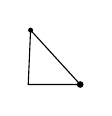
\begin{tikzpicture}[scale=.6]
\draw (0,0)--(.05,1.15)--(1.1,0)--cycle;
\fill (.05,1.15) circle (1.5pt); \fill (1.1,0) circle (2pt);
\end{tikzpicture}}
\[
\left\{(x_0-x_n;y)\ \middle|\ 
\left\{\begin{array}{l}
x_i\geq0\qquad\sum x_i=1\\
y\unsure{-}\displaystyle\sum_{0\leq i\leq n}a_i x_i=0
\end{array}\right.\right\}\in M_{n+2}
\]
si les $\{a_i\}\in M_1$

\margin{UNIVERSITE DES SCIENCES ET TECHNIQUES\\
DU LANGUEDOC\\
---\\
INSTITUT DE MATHEMATIQUES\\
Place Eugène Bataillon\\
34060 MONTPELLIER CEDEX\\
---\\
Montpellier, le}

\margin{66}

\scanpage{66}
\diagram{\begin{tikzcd}[ampersand replacement=\&]
E\arrow[dd,no head]\&\operatorname{Grass}_n(E)\arrow[ddl]\&\Sigma_{n,\sigma}(E)\arrow[l]\arrow[d]\arrow[dl]\\
\&\operatorname{Drap}(N)\arrow[u]\arrow[r,"{\deleted{\longrightarrow}}" description,draw=none]\&D_\sigma(E)\arrow[dll]\\
S\&\&
\end{tikzcd}}
\[
H^\bullet(S)[c_{\unsure{i}}^{\unsure{*}}(M),c_j(N)]/
\bigl((\textstyle\sum c_i(M))(\textstyle\sum c_j(N))=\textstyle\sum_h c_h(E)\bigr)
\]
\[
\xi_1-\xi_m\qquad c_1(N)-c_d(N)
\]
\[
\left(\prod_{1\leq i\leq m}(1+\xi_i)\right)
\sum_{0\leq j\leq d}c_j(N)
=\sum_{0\leq h\leq N}c_h(E)
\]
\diagram{\begin{tikzcd}[ampersand replacement=\&]
E\arrow[d,no head]\&E'\arrow[d,no head]\\
S\arrow[r,no head]\&S'=D_\sigma(E)
\end{tikzcd}}

\diagram{\begin{tikzcd}[ampersand replacement=\&]
X\arrow[r,hook,"{i}"]\arrow[d,"{p}"']\&Y\arrow[d,"{p'}"]\\
Z\arrow[r,hook,"{i'}"']\&S
\end{tikzcd}}
comm

$\unsure{d|a})$ $S=\operatorname{Im}i'\vee\operatorname{Im}p'$

i.e. $Z\amalg Y\longrightarrow S^{\deleted{\unsure{f}}}$ épi effectif

$\unsure{a})$ $i'$ mono

b) carré cartésien i.e. $X=p'^{-1}(Z)$

$\unsure{c})$ $Y\times_S Y=\Delta_Y\vee(X\times_Z X)$

$\Longrightarrow S\overset{\sim}{\longleftarrow}Y\amalg_X Z$

\[
(Z\amalg Y)\times_S(Z\amalg Y)=Z\amalg X\amalg X\amalg(Y\times_S Y)
\]
\diagram{\begin{tikzcd}[ampersand replacement=\&]
Z\amalg X\amalg X\amalg(Y\times_S Y)\arrow[r,shift left]\arrow[r,shift right]\&Z\amalg Y\arrow[r]\&S
\end{tikzcd}}
\diagram{\begin{tikzcd}[ampersand replacement=\&]
Z\amalg X\amalg X\amalg[(X\times_Z X)\amalg\Delta_Y]\arrow[r,shift left]\arrow[r,shift right]
\&Z\amalg Y\arrow[r]\arrow[dr,"{(f,g)}"']\&S\arrow[d,dashed]\\
\&\deleted{Z\amalg Y\longrightarrow S}\&T
\end{tikzcd}}

\figure{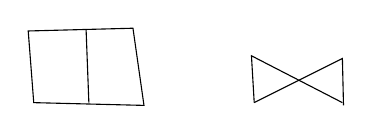
\begin{tikzpicture}[scale=.7]
\draw (0,0)--(-.1,1.3)--(1.8,1.35)--(2,-.05)--cycle;
\draw (1,0)--(.95,1.32);
\draw (4,0)--(3.95,.85)--(5.6,0);
\draw (4,0)--(5.6,.8)--(5.62,-.05);
\end{tikzpicture}}

\margin{67}

\scanpage{67}
$e\longrightarrow I^n$
\[
(\varepsilon_1-\varepsilon_n)
\]
\[
(\varepsilon_1,-\varepsilon_n,x_{n+1}-x_{n+p})
\]
\diagram{\begin{tikzcd}[ampersand replacement=\&]
I^{n+p}\arrow[d,"{x_1-x_n}"]\\ I
\end{tikzcd}}
\figure{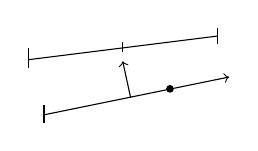
\begin{tikzpicture}
\draw (0,1)--(2.4,1.3); \draw (0,.9)--(0,1.15);
\draw (2.4,1.2)--(2.4,1.4); \draw (1.2,1.1)--(1.2,1.23);
\draw[->] (.2,.3)--(2.55,.78); \draw (.2,.2)--(.2,.43);
\fill (1.8,.63) circle (1.4pt); \draw[->] (1.3,.52)--(1.2,.98);
\end{tikzpicture}}
$(x,y)$\\
$(x',y')$\\
$(x,xy)=(x',x'y')$\\
$\boxed{x=x'}$\\
$xy=x'y'\qquad x=0$\\
$\deleted{x(y-y')=0}$

\diagram{\begin{tikzcd}[ampersand replacement=\&]
I^p\arrow[r]\arrow[d]\&I^{n+p}\arrow[d]\\
\left(\prod_{i\leq n}(\varepsilon_i\times I)\right)^p\times\unsure{e}
\arrow[r,hook]\&(I\times I)^{n\times p}\times I^n
\end{tikzcd}}

$\unsure{x_{ij}}\longleftarrow{}$\\
$f_1,-,f_n\qquad g_1-g_p$\\
$f_i g_j\qquad f'\qquad x_i,x_j$

\diagram{\begin{array}{c}
\boxed{\begin{tikzcd}[ampersand replacement=\&,column sep=large]
\varepsilon_i\times I\arrow[r,hook]\&I\times I
\end{tikzcd}}\\[-4pt]
\begin{tikzcd}[ampersand replacement=\&,column sep=large]
{}\arrow[d]\&{}\arrow[d,"{(x,y)\mapsto(x,xy)}"]\\
e\arrow[r]\&I\times I
\end{tikzcd}
\end{array}}

\diagram{\begin{tikzcd}[ampersand replacement=\&]
I^{n+p}\arrow[d,"{(f_i,g_j)}"']\arrow[dr]\&\\
(\unsure{I^n|I}\times I)^{np}\times\&I^n
\end{tikzcd}}
$f:$ \figure{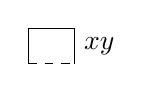
\begin{tikzpicture}[scale=.45]\draw (0,0)--(0,1)--(1.3,1)--(1.3,0);\draw[dashed](0,0)--(1.3,0);\node[right]at(1.3,.5){$xy$};\end{tikzpicture}}

\diagram{\begin{tikzcd}[ampersand replacement=\&]
I^p\arrow[r]\arrow[d]\&I^{n+p}\arrow[d]\\
(\unsure{e}\times I)^{np}\times\unsure{e}\arrow[r,hook]\&(I\times I)^{np}\times I^n
\end{tikzcd}}
\[
(\unsure{e}\times I)^{np}\subset(I\times I)^{np}
\]
a) $0y=0$

\deleted{Dear Fujii Guruji,\\
Please accept my most cordial\\
wishes of welcome in France\\
and of a very happy stay in\\
Paris,}

\diagram{\begin{tikzcd}[ampersand replacement=\&]
X\arrow[r,hook]\arrow[d]\arrow[dr]\&Y\arrow[d]\\
Z\arrow[r,hook]\&I^m
\end{tikzcd}}
comm

\diagram{\begin{tikzcd}[ampersand replacement=\&]
X\arrow[r,hook]\arrow[d]\&Y\arrow[d,"{\varphi=(\varphi_1-\varphi_n)}"]\\
e\arrow[r]\&I^n
\end{tikzcd}}
\deleted{\diagram{\begin{tikzcd}[ampersand replacement=\&]
X\arrow[r,hook]\arrow[d]\&Y\arrow[d,"{\varphi_1-\varphi_{p+n}}"]\\
I^p\arrow[r,hook]\&I^{p+n}
\end{tikzcd}}}
\[
Y\lhook\joinrel\longrightarrow I^p
\qquad \psi=(\psi_1-\psi_p)
\]
\[
\underbrace{(\varphi_i,\psi_j)}_{\chi_{ij}}:Y\longrightarrow(I\times I)^{n\times p}
\]
\deleted{$(\varphi_i,\psi_j)$ se}
$\chi_{ij}|X$ se factorise par $e_i\times I\subset I\times I$

\diagram{\begin{tikzcd}[ampersand replacement=\&]
X\arrow[r,hook]\arrow[d]\&Y\arrow[d]\\
X'=I^p\arrow[r,hook]\arrow[d]\&Y'=I^{n+p}\arrow[d]\\
e\arrow[r,hook]\&S
\arrow[phantom,from=1-1,to=2-2,"{\times}" description]
\arrow[phantom,from=2-1,to=3-2,"{\times}" description]
\end{tikzcd}}
\diagram{\begin{tikzcd}[ampersand replacement=\&]
Y\times Y\arrow[d]\&Y\times_S Y\arrow[l]\arrow[d]\\
Y'\times Y'\arrow[r]\&Y'\times_S Y'
\end{tikzcd}}
$\deleted{\longrightarrow Y\times_{Y'}Y\longrightarrow Y}$
\[
=\overbrace{(\unsure{Y}\times_{Y'}Y)}^{\Delta_{Y/Y'}}\vee(X\times X)
\]
\[
\unsure{\ne}\qquad
\text{``}\Delta_{Y'}\vee(X'\times X')
\]
$I^{\unsure{p}}\ --\ I^{n+p}$\\
$\deleted{\unsure{e\times e\times I^p}}$

\margin{68}

\scanpage{68}
\diagram{\begin{tikzcd}[ampersand replacement=\&]
X\arrow[r,hook,"{i}"]\arrow[d,leftrightarrow,"{p}"']\&Y\arrow[d,"{?}"]\\
Z\arrow[r,hook,"{?}"']\&I^n
\end{tikzcd}}
avec a) b) c)

$f_1-f_p:Z-I\qquad Z\to I^p$ mono

$f_\alpha\circ p=g_\alpha\circ i\ /\ \unsure{f_1-f_p|g_1-g_p}:Y-I$

OK pour a)

$Z\xrightarrow{0}I^{\unsure{q}}$\\
$f_{p+1}-f_{p+q}=0$

$f_{p+\beta}\circ p=0$

$g_{p+\beta}\circ i=0\qquad\displaystyle\bigcap_{1\leq\beta\leq q}g_{p+\beta}^{-1}(0)=X$ i.e.

carré
\diagram{\begin{tikzcd}[ampersand replacement=\&]
X\arrow[r,hook]\arrow[d]\&Y\arrow[d]\\
e\arrow[r]\&I^q
\end{tikzcd}}
cart.

OK pour b)

$Y\times_{I^q}Y=\Delta_Y\vee(X\times X)$

\diagram{\begin{tikzcd}[ampersand replacement=\&]
X\arrow[r,hook,"{i}"]\arrow[d,"{p}"']\&Y\arrow[d]\\
Z\arrow[r]\arrow[d]\&I^{p+q}=S\arrow[d]\\
e\arrow[r]\&I^q=S'
\end{tikzcd}}
\diagram{\begin{tikzcd}[ampersand replacement=\&]
Y\times_S Y\arrow[r,leftrightarrow]\arrow[d,leftrightarrow]\&
\deleted{\unsure{Y\times_{S'}S}}\ S\arrow[d,leftrightarrow,"{\delta}"]\\
Y\times_{S'}Y\arrow[r,leftrightarrow]\arrow[d,equal]\&S\times_{S'}S\\
\Delta_Y\vee X\times X\&
\end{tikzcd}}

\margin{69}

\scanpage{70}
\mspage{1}
\margin{71}
\uline{1}. Soit $R$ un ensemble (ce sera bientôt $\mathbb R$). \deleted{\unsure{Soit C}}
Soit pour \deleted{tout} $n\in\mathbb N$, $C_n\unsure{\in|\subset}R^n$. On suppose

\textcircled{a} $C_n$ stable par $\mathfrak S_n$

\textcircled{b} Soient $p,n\in\mathbb N$, $p\leq n$, considérons
\[
\varphi_{p,n}:R^n\longrightarrow R^p,\qquad
(x_1,--x_n)\longmapsto(x_1,--,x_p)
\]
alors $\varphi_{p,n}(X)\in C_p$ si $X\in C_n$

\textcircled{c} Soient $p_1,p_2,--,p_n\in\mathbb N$, \inserted{$p_*=(p_1,--p_n)$}, considérons
\[
R^n\xrightarrow{\varphi_{p_*}}R^{\overbrace{p_1+\cdots+p_n}^{p}}
\]
\[
x_1,-x_n\longmapsto
(\underbrace{x_1,--x_1}_{p_1\ \mathrm{fois}},--,\underbrace{x_n,--x_n}_{p_n\ \mathrm{fois}})
\]
\deleted{d) $\exists n$ tel que $C_n\ne\varnothing$ $(\Leftrightarrow C_0\ne\varnothing$}
alors $\varphi_{p_*}(X)\in C_p$ si $X\in C_n$

\textcircled{d} Si $X\in C_m$, $Y\in C_n$, alors $X\times Y\in C_{m+n}$

\uline{NB} Il revient au $=$, pour tt ens. fini $I$, de se donner \deleted{\unsure{le}} $C_I\subset\mathcal P(R^I)$, de telle façon que pour tt $\alpha:I\to J$ ($I,J$ ens finis) d'où $\alpha^*:R^J\to R^I$, on ait $\alpha^*(X)\in C_I$ pour $X\in C_J$, et que $X\in C_I$, $Y\in C_J\Rightarrow X\times Y\in C_{I\amalg J}$.

\uline{Prop} Si $X,Y\in C_n$, alors $X\cap Y\in C_n$

\uline{Déf} Soit $X\in C_I$, $Y\in C_{\unsure{J|Y}}$, $f:X\to Y$, d'où $\Gamma_f\subset X\times Y\subset R^{I\amalg J}$. On dit que $f$ est un $C_*$-morphisme si $\Gamma_f\in C_{I\amalg J}$.
\inserted{[NB. ne dépend que du composé \deleted{et non de}
\diagram{\begin{tikzcd}[ampersand replacement=\&]
X\arrow[r]\arrow[rr,bend right]\&Y\arrow[r,hook]\&R^J
\end{tikzcd}}]}

\deleted{\uline{Prop} Soit $X,Y\in C_n$, alors $X\cap Y\in C_n$}

\uline{Prop} a) Si $X\in C_I$, $\operatorname{id}_X$ est $C_*$-morphisme

b) Le composé de deux $C_*$-morphismes est \unsure{itou}.

c) \deleted{Soit} $f:X\overset{\deleted{\unsure{\text{est}}}}{\longrightarrow}Y$ une bijection. Pour que $f$ soit un $C_*$-morphisme, il f. et s. que $f^{-1}$ le soit.

d) Soient $X\in C_I$, $Y\in C_J$, $Z\in C_K$, $g:X\to Y$, $h:X\to Z$, d'où $f=(g,h):X\to Y\times Z$ \deleted{$\unsure{\in C}$} (où $Y\times Z\in C_{J\amalg K}$).
Alors $f$ est un $C_*$-morphisme ssi $g$ et $h$ le sont.

\margin{e) Soit $\alpha:\deleted{\unsure{E}}\inserted{I}\to J$, d'où $\alpha^*:R^J\to R^I$, soit $X\in C_J$, d'où $Y=\alpha^*(X)\in C_I$. Alors $\alpha^*|X:X\to Y$ est un $C_*$-morphisme.
f) Si $X\subset Y$, $X,Y\in C_I$, alors l'inclusion $X\lhook\joinrel\longrightarrow Y$ est un $C_*$-morphisme.}

\margin{g) Si $f:X\to Y$ est un $C_*$-morphisme, $X\in C_n$, $Y\in C_m$, alors $f(X')\in C_m$ pour $X'\subset X$, $X'\in C_n$.
h) Si $f:X\to Y$ comme dessus, alors $f^{-1}(Y')\in C_n$ si $Y'\subset Y$, $Y'\in C_m$.}

\uline{Définition} \deleted{\unsure{Une}} Structure \inserted{$T$ de $C_*$-modèle} sur un ens \deleted{\unsure{E}} est la donnée, pour \deleted{tout} $n\in\mathbb N$ d'un ens $T_n$ d'applications injectives de $E$ dans $\mathbb R^n$, telle que

\scanpage{71}
a) $\exists n\in\mathbb N$ tel que $T_n\ne\varnothing$

\inserted{b) $\forall m\in\mathbb N$ et $v\in T_m$, on a $v(E)\in C_m$}

$\unsure{c|b})$ Si \deleted{$\unsure{u\in T_n}$} $(u:E\to R^n)\in T_n$, et si $v:E\lhook\joinrel\longrightarrow R^m$, alors $v\in T_m$ ssi $1^\circ)$ $v(E)\in C_m$ et $2^\circ)$
\[
vu^{-1}:\underset{\cap\,R^n}{u(E)}
\longrightarrow\underset{\cap\,R^m}{v(E)}
\]
est un $C_*$-morphisme

\margin{Cette structure peut aussi être définie par l'ens $\Sigma$ des $C_*$-morphismes de $E$ dans $R$, avec l'axiome suivant
a) $\exists J\subset\Sigma$, partie finie, telle que $E\to R^J$ can. soit injectif, et ait une image $X\in C_J$.
b) On peut choisir $J$ tel que $\forall f:E\to R$, on ait $f\in\Sigma$ ssi le composé
\diagram{\begin{tikzcd}[ampersand replacement=\&]
X\arrow[r,"{\sim}"]\&E\arrow[r,"{f}"]\&R
\end{tikzcd}}
est $C_*$-morphisme,
\inserted{inverse de $E\overset{\sim}{\to}X$}.}

\uline{Ex} Si $n\in\mathbb N$, $X\subset R^n$ avec $X\in C_n$, alors $X$ est muni d'une $C_*$-structure canonique.

\uline{Déf} Soient $X,Y$ deux $C_*$-modèles. Une application $f:X\to Y$ est dite un $C_*$-morphisme si ---

\uline{Prop} Les \deleted{dé} $C_*$-modèles, et $C_*$-morphismes, forment une catégorie (pour la composition ensembliste des morphismes).
Dans cette catégorie, les produits \deleted{finis} de deux objets existent.
Un morphisme de $C_*$-modèles est un iso. ssi il est bijectif.

\uline{Prop} Conditions équivalentes sur $C_*$

a) \deleted{$\unsure{C_0\ne\varnothing}$} $\exists n\in\mathbb N$ et $X\in C_n$, tel que $X\ne\varnothing$

b) $R^0\in C_0$

c) La catégorie des $C_*$-modèles admet des objets de cardinal $1$ (i.e. sur un ens. à $1$ élément, existe une structure de $C_*$-modèle)

Alors les \deleted{\unsure{modè}} $C_*$-modèles \unsure{uniponctuels} sont des objets finaux de la catégorie des $C_*$-modèles.

Dorénavant, on supposera cette condition, sous la forme plus forte

\textcircled{5} \deleted{$R^0\in C_0$}
\inserted{$\forall n\in\mathbb N$, on a}
\[
R^n=\bigcup_{X\in C_n}X
\]

\margin{On définit la notion de $C_*$-partie d'un $C_*$-modèle, de façon unique, de façon que ça commute au ``transport de structure'' et ait Si $X\in C_n$ ($n\in\mathbb N$), alors pour $Y\subset X$, $Y$ est une $C_*$-partie du $C_*$-modèle $X$ ssi $Y\in C_n$.
Ceci dit, pour un morphisme de modèles, l'image directe ou inverse d'une $C_*$-partie est itou.
Notion de $C_*$-str. induite.}

\margin{72}

\scanpage{72}
2. Je suppose maintenant que $R$ est un esp. top \inserted{séparé} et je suppose

\textcircled{\unsure{7|6}} Si \inserted{$n\in\mathbb N$,} $X\in C_n$, $X$ est \uline{compact}.

Cela implique que si $X\in C_n$, $Y\in C_p$, alors tt $C_*$-morphisme de $X$ dans $Y$ est \uline{continu}, que les $C_*$-modèles sont de façon canonique munis d'une structure d'espace compact, \deleted{qui} \unsure{sorte qu'on trouve} un foncteur canonique
\[
(C_*\text{-modèles})\longrightarrow\text{espaces compacts}.
\]

Je suppose de plus

\textcircled{8} Si $n\in\mathbb N$, $X\in C_n$, et $x\in X$, alors \deleted{$\forall$ voisinage $V$ de \unsure{$x$}; les}
\deleted{$V\in C_n$ qui sont un voisinage de $x$ dans $X$, $\exists Y$}
les $Y\in C_n$ qui \inserted{$\subset X$} sont un voisinage de $x$ \inserted{dans $X$} forment un syst. fond. de voisinages de $x$ dans $X$.

[Il suffit que \deleted{\unsure{tous}} les intérieurs des $X\in C_n$ forment une base de la topologie de $R^n$]
\margin{C'est ce qu'on supposera}

Alors, les \inserted{$C_*$-}morphismes d'un $C_*$-modèle $X$ dans un autre $Y$ sont les sections d'un faisceau -- le faisceau des germes de $C_*$-morphismes de $X$ dans $Y$.
Idem pour les $C_*$-morphismes dans $R$ (ou dans un $R^I$).
La connaissance du faisceau des $C_*$-morphismes d'un modèle $X$ (donné comme espace cpt) dans $R$, \inserted{\unsure{connu pour ss-faisceau de celui des appl. cont. de $X$ dans $R$|contt pour ss-faisceau de celui des appl. cont. de $X$ dans $R$}}, redonne la \inserted{$C_*$-}structure du modèle.

$C_*$-espace : espace loc.$^{\mathrm t}$ compact, muni d'un sous-faisceau du faisceau des appl. continues à val. dans $R$, tel que tt pt ait un voisinage cpt qui, pour la structure induite, soit un $C_*$-modèle ---

\margin{73}

\scanpage{73}
\mspage{2}
Considérons la condition

\textcircled{6} $\forall n\in\mathbb N$, $C_n$ stable par réunions finies $(\Rightarrow\varnothing\in C_n)$

On en conclut

\uline{Prop} Soit $X$ un $C_*$-modèle, $(X_i)_{i\in I}$ une \deleted{un} famille finie de $C_*$-parties de $X$, avec $X=\bigcup X_i$, $f:X-Y$ une application de $X$ dans un $C_*$-modèle $Y$.
Alors $f$ est un $C_*$-morph. ssi $\forall i\in I$, $f|X_i$ l'est.

\uline{Corollaire} Dans la cat. des $C_*$-modèles, $X$ est la somme amalgamée des $X_i$, sur les $X_i\cap X_j$.

\uline{Question} Soit un diagramme
\diagram{\begin{tikzcd}[ampersand replacement=\&]
\&Z\arrow[dl,hook]\arrow[dr,hook]\&\\
X\&\&Y
\end{tikzcd}}
dans la catégorie des $C_*$-modèles, y a-t-il une somme amalgamée ? O.K. Si on \deleted{prend} \uline{la condition} suivante :
$\forall n\in\mathbb N$, $X,Y\in C_n$, $Y\subset X$, et tt $C_*$-morphisme $f_Y:Y-R$; $\exists$ $C_*$-morphisme $f_X:X-R$ qui le prolonge.

\margin{?\\ à tirer au clair...}
\margin{74}

\cotefile{153}
\scanpage{1}
\figure{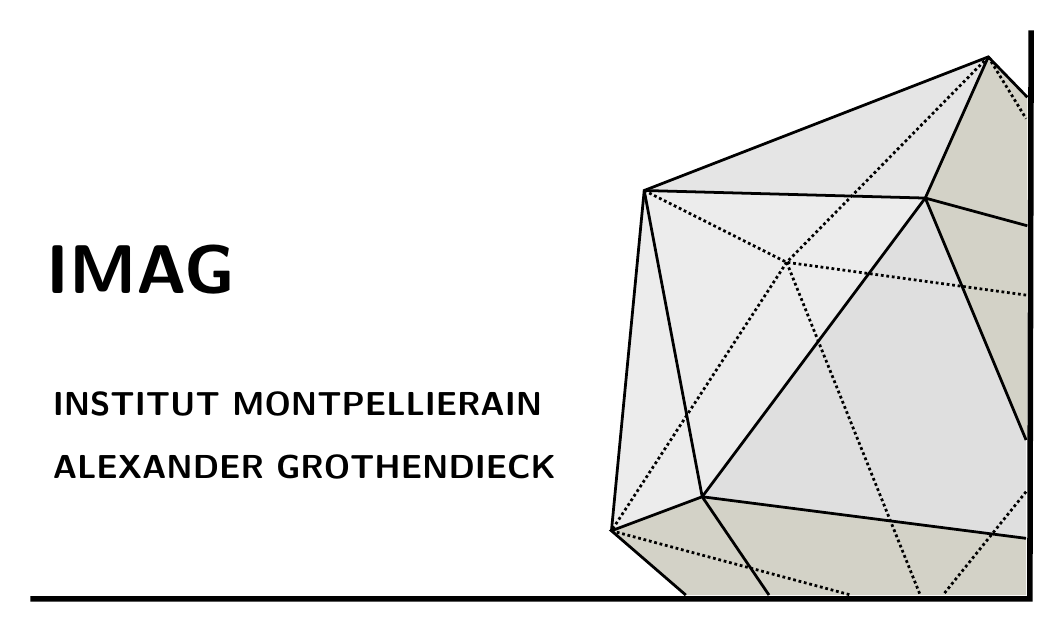
\begin{tikzpicture}[x=.016cm,y=.016cm]
\node[anchor=west,font=\sffamily\bfseries\fontsize{60}{65}\selectfont] at (15,285){IMAG};
\node[anchor=west,font=\sffamily\bfseries\large] at (20,179){INSTITUT MONTPELLIERAIN};
\node[anchor=west,font=\sffamily\bfseries\large] at (20,129){ALEXANDER GROTHENDIECK};
\fill[gray!20] (497,348)--(770,454)--(720,342)--cycle;
\fill[gray!15] (497,348)--(720,342)--(543,105)--(471,78)--cycle;
\fill[gray!25] (720,342)--(800,150)--(800,72)--(543,105)--cycle;
\fill[yellow!12!gray!45] (770,454)--(801,422)--(801,150)--(720,342)--cycle;
\fill[yellow!12!gray!45] (471,78)--(543,105)--(800,72)--(800,27)--(530,27)--cycle;
\draw[line width=1pt] (471,78)--(497,348)--(770,454)--(801,422);
\draw[line width=1pt] (497,348)--(720,342)--(801,320);
\draw[line width=1pt] (770,454)--(720,342)--(800,150);
\draw[line width=1pt] (497,348)--(543,105)--(596,27);
\draw[line width=1pt] (720,342)--(543,105)--(471,78)--(530,27);
\draw[line width=1pt] (543,105)--(800,72);
\draw[densely dotted,line width=1pt] (497,348)--(610,291)--(800,265);
\draw[densely dotted,line width=1pt] (770,454)--(610,291)--(471,78);
\draw[densely dotted,line width=1pt] (610,291)--(716,27);
\draw[densely dotted,line width=1pt] (471,78)--(661,27);
\draw[densely dotted,line width=1pt] (800,109)--(734,27);
\draw[densely dotted,line width=1pt] (770,454)--(800,405);
\draw[line width=2pt] (10,24)--(803,24)--(804,475);
\end{tikzpicture}}

\scanpage{2}
\mspage{1}
$k_0$ anneau de base (cas important : $k_0=\mathbb Z$)

$\Omega_0$ \deleted{$k_0\langle T\rangle$} $k_0$-algèbre, contient l'élément $T$, d'où
\[
k_0[T]\xrightarrow{\varphi}\deleted{k_0\langle T\rangle}\ \Omega_0
\]
Opération
\[
\deleted{k_0\langle T\rangle\times k_0\langle T\rangle}
\inserted{\Omega_0\times\Omega_0}
\longrightarrow\deleted{k_0\langle T\rangle}\ \Omega_0
\]
\[
(F,G)\longmapsto F\circ G
\]
\begin{align*}
\text{a)}\quad &(F\circ G)\circ H=F\circ(G\circ H)\\
\text{b)}\quad &T\circ F=F\circ T=F\\
\text{c)}\quad &\varphi(\underbrace{F\circ G}_{\text{composition habituelle}})=\varphi(F)\circ\varphi(G)
\end{align*}
\margin{ainsi $\varphi$ est défini en termes de l'opération $F\circ G$ sur $\Omega_0$}
d) $F\longmapsto F\circ G:k_0\langle T\rangle\to k_0\langle T\rangle$ est \deleted{\unsure{un}}\inserted{morphisme de} $k_0$-alg.

$\left[\begin{array}{ll}
\text{e)}&F\circ(G+G')=\\
\text{f)}&F\circ(GG')=
\end{array}\right.$

\deleted{\unsure{g)}} g: $F\circ\lambda1=F(\lambda).1$\\
où $\Omega_0$ opère sur $k_0$ par $(F,\lambda)\mapsto F(\lambda)$ $\big]$

\margin{$F(T)=a_0+a_1T+\unsure{a_n|a_2}\dfrac{T^{\unsure{n|2}}}{\unsure{n!|2!}}+\cdots$\\
$\dfrac{T(T-1)}2$}
\margin{Multip. $W(\Omega_0)\times W(\Omega_0)\to\unsure{W\Omega_0|W(\Omega_0)}$}

$\Omega_0$ $k_0$-algèbre (\unsure{évt.} sans unité)\\
$\in$\\
$T$

$W(\Omega_0)\times W(\Omega_0)-W(\Omega_0)$

$\deleted{\unsure{E}}\qquad k_0\qquad A\quad k_0$-algèbre comm. ``sans unités''

$E^1\qquad\mathfrak S\qquad\deleted{\uline{\operatorname{End}}(M)}\quad W(A)\quad\unsure{\underline{\mathcal O}_{k_0}|\underline O_{k_0}}$-algèbre

$\uline{\operatorname{End}}W(A)$ : \deleted{deux}\inserted{une} structures de \inserted{$\unsure{\underline{\mathcal O}_{k_0}|\underline O_{k_0}}$-}algèbre
\[
(\lambda F)(x)=\lambda F(x)
\]
\[
(F+G)(x)=F(x)+G(x)
\]
\[
(FG)(x)=F(x).G(x)
\]
et une \inserted{autre} structure \deleted{de $k_0$-algèbre} \inserted{d'anneau} : gr. $=$ structure \deleted{additive} \inserted{$G_a$-loi}, et comme multiplication
\[
(F\circ G)(x)=F(G(x))
\]

$W(\Omega_0)\longrightarrow\uline{\operatorname{End}}W(A)$

$F(x+\unsure{\cdot}$

$\Omega_0$ opère sur $A$

$W(\Omega_0)\ --\ W(A)$

$\deleted{F(x+y)=\Delta F(x\unsure{;}}$\\
$\Omega_0\otimes\Omega_0\qquad A\otimes A$

\diagram{\begin{tikzcd}[ampersand replacement=\&]
k_0\arrow[d,no head]\\
\mathbb Z\arrow[r,no head]\&{}
\end{tikzcd}}

\margin{1}

\scanpage{3}
\diagram{\begin{array}{l}
\texttt{\ \ \ \ \ \ \ \ \ \ \ 00000000\ \ \ \ \ \ 00000000\ \ \ \ \ \ \ \ \ \ 444\ \ \ \ \ \ 9999999999} \\
\texttt{\ \ \ \ \ \ \ \ \ 0000000000\ \ \ \ 0000000000\ \ \ \ \ \ \ \ 4444\ \ \ \ \ 999999999999} \\
\texttt{\ \ \ \ \ \ \ 00\ \ \ \ \ \ 0000\ \ 00\ \ \ \ \ \ 0000\ \ \ \ \ \ \ 44\ 44\ \ \ \ 99\ \ \ \ \ \ \ \ 99} \\
\texttt{\ \ \ \ \ \ 00\ \ \ \ \ 00\ 00\ \ 00\ \ \ \ \ 00\ 00\ \ \ \ \ \ 44\ \ 44\ \ \ 99\ \ \ \ \ \ \ \ 99} \\
\texttt{\ \ \ \ \ 00\ \ \ \ 00\ \ 00\ \ 00\ \ \ \ 00\ \ 00\ \ \ \ \ \ 44\ \ \ 44\ \ 99\ \ \ \ \ \ \ \ 99} \\
\texttt{\ \ \ \ 00\ \ \ 00\ \ \ 00\ \ 00\ \ \ 00\ \ \ 00\ \ \ \ \ 44444444444\ 999999999999} \\
\texttt{\ \ \ 00\ \ 00\ \ \ \ 00\ \ 00\ \ 00\ \ \ \ 00\ \ \ \ 444444444444\ 999999999999} \\
\texttt{\ \ 00\ 00\ \ \ \ \ 00\ \ 00\ 00\ \ \ \ \ 00\ \ \ \ \ \ \ \ \ \ \ 44\ \ \ \ \ \ \ \ \ \ \ 99} \\
\texttt{\ 0000\ \ \ \ \ \ 00\ \ 0000\ \ \ \ \ \ 00\ \ \ \ \ \ \ \ \ \ \ 44\ \ \ \ \ \ \ \ \ \ \ 99} \\
\texttt{000\ \ \ \ \ \ \ 00\ \ 000\ \ \ \ \ \ \ 00\ \ \ \ \ \ \ \ \ \ \ 44\ \ \ \ \ 99\ \ \ \ 99} \\
\texttt{0000000000\ \ \ \ 0000000000\ \ \ \ \ \ \ \ \ \ \ \ 44\ \ \ \ \ 999999999999} \\
\texttt{00000000\ \ \ \ \ \ 00000000\ \ \ \ \ \ \ \ \ \ \ \ \ 44\ \ \ \ \ \ 9999999999}
\end{array}}

\diagram{\begin{array}{l}
\texttt{PPPPPPPPPPP\ \ \ RRRRRRRRRRR\ \ \ EEEEEEEEEEEE\ \ DDDDDDDDD\ \ \ \ \ OOOOOOOOOOOO\ \ NN\ \ \ \ \ \ \ \ NN\ \ TTTTTTTTTTTT\ \ \ AAAAAAAAAA} \\
\texttt{PPPPPPPPPPPP\ \ RRRRRRRRRRRR\ \ EEEEEEEEEEEE\ \ DDDDDDDDDD\ \ \ \ OOOOOOOOOOOO\ \ NNN\ \ \ \ \ \ \ NN\ \ TTTTTTTTTTTT\ \ AAAAAAAAAAAA} \\
\texttt{PP\ \ \ \ \ \ \ \ PP\ \ RR\ \ \ \ \ \ \ \ RR\ \ EE\ \ \ \ \ \ \ \ \ \ \ \ DD\ \ \ \ \ \ \ DD\ \ \ OO\ \ \ \ \ \ \ \ OO\ \ NNNN\ \ \ \ \ \ NN\ \ \ \ \ \ \ TT\ \ \ \ \ \ \ AA\ \ \ \ \ \ \ \ AA} \\
\texttt{PP\ \ \ \ \ \ \ \ PP\ \ RR\ \ \ \ \ \ \ \ RR\ \ EE\ \ \ \ \ \ \ \ \ \ \ \ DD\ \ \ \ \ \ \ \ DD\ \ OO\ \ \ \ \ \ \ \ OO\ \ NN\ NN\ \ \ \ \ NN\ \ \ \ \ \ \ TT\ \ \ \ \ \ \ AA\ \ \ \ \ \ \ \ AA} \\
\texttt{PP\ \ \ \ \ \ \ \ PP\ \ RR\ \ \ \ \ \ \ \ RR\ \ EE\ \ \ \ \ \ \ \ \ \ \ \ DD\ \ \ \ \ \ \ \ DD\ \ OO\ \ \ \ \ \ \ \ OO\ \ NN\ \ NN\ \ \ \ NN\ \ \ \ \ \ \ TT\ \ \ \ \ \ \ AA\ \ \ \ \ \ \ \ AA} \\
\texttt{PPPPPPPPPPPP\ \ RRRRRRRRRRRR\ \ EEEEEEEE\ \ \ \ \ \ DD\ \ \ \ \ \ \ \ DD\ \ OO\ \ \ \ \ \ \ \ OO\ \ NN\ \ \ NN\ \ \ NN\ \ \ \ \ \ \ TT\ \ \ \ \ \ \ AAAAAAAAAAAA} \\
\texttt{PPPPPPPPPPP\ \ \ RRRRRRRRRRR\ \ \ EEEEEEEE\ \ \ \ \ \ DD\ \ \ \ \ \ \ \ DD\ \ OO\ \ \ \ \ \ \ \ OO\ \ NN\ \ \ \ NN\ \ NN\ \ \ \ \ \ \ TT\ \ \ \ \ \ \ AAAAAAAAAAAA} \\
\texttt{PP\ \ \ \ \ \ \ \ \ \ \ \ RR\ \ \ \ RR\ \ \ \ \ \ EE\ \ \ \ \ \ \ \ \ \ \ \ DD\ \ \ \ \ \ \ \ DD\ \ OO\ \ \ \ \ \ \ \ OO\ \ NN\ \ \ \ \ NN\ NN\ \ \ \ \ \ \ TT\ \ \ \ \ \ \ AA\ \ \ \ \ \ \ \ AA} \\
\texttt{PP\ \ \ \ \ \ \ \ \ \ \ \ RR\ \ \ \ \ RR\ \ \ \ \ EE\ \ \ \ \ \ \ \ \ \ \ \ DD\ \ \ \ \ \ \ \ DD\ \ OO\ \ \ \ \ \ \ \ OO\ \ NN\ \ \ \ \ \ NNNN\ \ \ \ \ \ \ TT\ \ \ \ \ \ \ AA\ \ \ \ \ \ \ \ AA} \\
\texttt{PP\ \ \ \ \ \ \ \ \ \ \ \ RR\ \ \ \ \ \ RR\ \ \ \ EE\ \ \ \ \ \ \ \ \ \ \ \ DD\ \ \ \ \ \ \ DD\ \ \ OO\ \ \ \ \ \ \ \ OO\ \ NN\ \ \ \ \ \ \ NNN\ \ \ \ \ \ \ TT\ \ \ \ \ \ \ AA\ \ \ \ \ \ \ \ AA} \\
\texttt{PP\ \ \ \ \ \ \ \ \ \ \ \ RR\ \ \ \ \ \ \ RR\ \ \ EEEEEEEEEEEE\ \ DDDDDDDDDD\ \ \ \ OOOOOOOOOOOO\ \ NN\ \ \ \ \ \ \ \ NN\ \ \ \ \ \ \ TT\ \ \ \ \ \ \ AA\ \ \ \ \ \ \ \ AA} \\
\texttt{PP\ \ \ \ \ \ \ \ \ \ \ \ RR\ \ \ \ \ \ \ \ RR\ \ EEEEEEEEEEEE\ \ DDDDDDDDD\ \ \ \ \ OOOOOOOOOOOO\ \ NN\ \ \ \ \ \ \ \ \ N\ \ \ \ \ \ \ TT\ \ \ \ \ \ \ AA\ \ \ \ \ \ \ \ AA}
\end{array}}

\diagram{\begin{array}{l}
\texttt{****A\ \ \ END\ \ \ JOB\ \ \ 1\ \ \ PREDONTA\ \ \ \ \ \ \ \ \ \ \ \ \ \ \ \ \ \ \ \ \ \ \ \ \ ROOM\ \ \ \ \ \ \ 5.14.26\ PM\ 19\ APR\ 82\ \ \ R6.PR1\ \ \ SYS\ JES2\ \ \ JOB\ \ \ 1\ \ \ END\ \ \ A****} \\
\texttt{****A\ \ \ END\ \ \ JOB\ \ \ 1\ \ \ PREDONTA\ \ \ \ \ \ \ \ \ \ \ \ \ \ \ \ \ \ \ \ \ \ \ \ \ ROOM\ \ \ \ \ \ \ 5.14.26\ PM\ 19\ APR\ 82\ \ \ R6.PR1\ \ \ SYS\ JES2\ \ \ JOB\ \ \ 1\ \ \ END\ \ \ A****} \\
\texttt{****A\ \ \ END\ \ \ JOB\ \ \ 1\ \ \ PREDONTA\ \ \ \ \ \ \ \ \ \ \ \ \ \ \ \ \ \ \ \ \ \ \ \ \ ROOM\ \ \ \ \ \ \ 5.14.26\ PM\ 19\ APR\ 82\ \ \ R6.PR1\ \ \ SYS\ JES2\ \ \ JOB\ \ \ 1\ \ \ END\ \ \ A****} \\
\texttt{****A\ \ \ END\ \ \ JOB\ \ \ 1\ \ \ PREDONTA\ \ \ \ \ \ \ \ \ \ \ \ \ \ \ \ \ \ \ \ \ \ \ \ \ ROOM\ \ \ \ \ \ \ 5.14.26\ PM\ 19\ APR\ 82\ \ \ R6.PR1\ \ \ SYS\ JES2\ \ \ JOB\ \ \ 1\ \ \ END\ \ \ A****} \\
\texttt{****A\ \ \ END\ \ \ JOB\ \ \ 1\ \ \ PREDONTA\ \ \ \ \ \ \ \ \ \ \ \ \ \ \ \ \ \ \ \ \ \ \ \ \ ROOM\ \ \ \ \ \ \ 5.14.26\ PM\ 19\ APR\ 82\ \ \ R6.PR1\ \ \ SYS\ JES2\ \ \ JOB\ \ \ 1\ \ \ END\ \ \ A****} \\
\texttt{****A\ \ \ END\ \ \ JOB\ \ \ 1\ \ \ PREDONTA\ \ \ \ \ \ \ \ \ \ \ \ \ \ \ \ \ \ \ \ \ \ \ \ \ ROOM\ \ \ \ \ \ \ 5.14.26\ PM\ 19\ APR\ 82\ \ \ R6.PR1\ \ \ SYS\ JES2\ \ \ JOB\ \ \ 1\ \ \ END\ \ \ A****}
\end{array}}

\[
n\in\mathbb N\qquad F_n(T)=\frac{T(T-1)-(T-n+1)}{n!}\in\mathbb Q[T]
\]
\[
(*)\quad F_m(T)F_n(T)=\sum_{0\leq p\leq m+n}\underbrace{c^p_{m,n}}_{\substack{\uparrow\\\mathbb Z}}F_p(T).
\]
\[
F_m(F_n(T))=\sum_{0\leq p\leq mn}d^p_{m,n}F_p(T)
\]
\[
\bigoplus\mathbb Z.F_n\subset\mathbb Q[T].
\]
est la $\mathbb Z$-algèbre \inserted{comm. avec $1$} engendrée par les $F_n$ $(n\in\mathbb N)$ \unsure{soumis|soumises} aux relations: $F_0=1$ et $(*)$ (on pose alors $F_1=T$),
\[
F_m(P(T)+Q(T))=\sum\unsure{\gamma^m_{ij}|\delta^m_{ij}}F_i(P(T))F_j(Q(T))
\]
\[
\delta:\Omega\longrightarrow\Omega\otimes_{\mathbb Z}\Omega
\]
\[
F_m(P(T)Q(T)=\sum\delta^m_{ij}(P(T))
\]
\[
F_m(x+y)
\]
\[
F_m(xy)
\]
\[
\sum\unsure{a_i|a_n}T^i\qquad a_i\in\mathbb Q
\]
\figure{\begin{tikzpicture}\draw[line width=1.2pt] (0,0)--(0,.35);\end{tikzpicture}}
\margin{2}

\scanpage{4}
\mspage{\textcircled{2}}
Soit \deleted{$k_0$ anneau intègre, $K_0$ son corps des fractions,}
Soit $k_0\subset K_0$ inclusion d'anneaux comm.
\[
\begin{gathered}
\Omega\subset K_0[T]\\
\Vert\\
\{F\in K_0[T]\mid F(\lambda)\in k_0\quad\forall\lambda\in k_0\}
\end{gathered}
\]
\margin{\diagram{\begin{tikzcd}[ampersand replacement=\&]
K_0[T]\arrow[r] \& \mathrm{Appl}(K_0,K_0)\\
\Omega\arrow[u,hook]\arrow[r,dashed] \& \mathrm{Appl}((K_0,k_0),(K_0,k_0))\arrow[u,hook]
\end{tikzcd}}}
Alors $\Omega$ est une sous-\inserted{$k_0$-}algèbre de $K_0[T]$, \uline{stable par $F\circ G$}.

$\Omega$ opère sur $k_0$, de façon que
\[
\left\{
\begin{aligned}
(F+G)(x)&=F(x)+G(x)\\
\deleted{(\unsure{\lambda F})(x)=\lambda\unsure{F(x)}}\quad
(\lambda F)(x)&=\lambda(F(x))\\
(FG)(x)&=F(x)G(x)\\
(F\circ G)(x)&=F(G(x))
\end{aligned}
\right.
\]

De plus, on aura
\[
F(x+y)\overset{?}{=}\sum G_i(x)H_i(y)
\]
\[
F(xy)\overset{?}{=}\sum J_\alpha(x)K_\alpha(y)
\]
\margin{OK si $\Omega$ est un $k_0$-module \uline{libre}}

\margin{\uline{Lemme} si $M$ est un $k_0$-module libre, alors le sous-ens.
$\Omega_M\subset K_0[T]\otimes_{K_0}M_{K_0}$
\deleted{\unsure{constitué des} \unsure{polyn.} $\unsure{F\in M_{K_0}}$}
formé des $F$ tels que $F(x)\in M$ $\forall x\in k_0$, s'identifie à
$\Omega\otimes_{k_0}M$}
\margin{où $\sum_iG_i\otimes_{k_0}H_i$ est un élément bien déterminé de $\Omega\otimes_{k_0}\Omega$
et $\sum J_\alpha\otimes_{k_0}K_\alpha$ est un él. bien déterminé de $\Omega\otimes_{k_0}\Omega$}

En effet, dans $K_0[X,Y]=K_0[X]\otimes_{K_0}K_0[Y]$, on aura
\[
F(X+Y)\overset{\mathrm{def}}{=}\underset{\longrightarrow}{\Delta_a F}(X,Y)
\]
\[
F(XY)\overset{\mathrm{def}}{=}\unsure{\Delta_m^*|\Delta_m}F(X,Y)
\]
\margin{polynôme en $X,Y$, coeff $\in K_0$, qui pour des val. $x,y\in k_0$ a des valeurs dans $k_0$\\
id.}

\hrule
\[
F\circ(P+Q)=\sum_i(G_i\circ P)(H_i\circ Q)
\]
\[
F\circ(PQ)=\sum(J_\alpha\circ P)(K_\alpha\circ Q)
\]
\[
F\circ\lambda T=\sum J_\alpha(\lambda)K_\alpha
\left(=\sum K_\alpha(\lambda)J_\alpha\right)
\]
\margin{3}

\scanpage{5}
\texttt{D A T A S E T S\quad P I C T U R E S}
\diagram{\begin{array}{l}
\unsure{\texttt{******************************************************************************************************************}} \\
\texttt{*\ \ \ \ \ \ \ \ \ \ \ \ \ \ *\ \ \ \ \ \ \ \ \ \ \ \ \ \ \ \ \ \ *\ \ \ \ \ \ \ \ *\ \ \ \ \ \ \ *\ \ \ \ \ \ \ \ \ \ \ \ \ *\ \ \ \ \ \ \ \ \ \ \ \ *\ \ \ \ \ *\ \ \ \ \ \ \ *\ \ \ \ \ \ \ \ *\ \ \ \ \ \ \ \ \ \ \ *} \\
\texttt{*\ \ \ DDNAME\ \ \ \ \ *\ DESTINATION\ \ \ \ \ \ *\ \ CLASS\ *COPIES\ *\ \ RECORDS-NB\ *\ \ BYTES-NB\ \ *FORM\ *\ FCB\ \ \ *\ \ UCS\ \ \ *SPIN\ \ HOLD\ *} \\
\texttt{*\ \ \ \ \ \ \ \ \ \ \ \ \ \ *\ \ \ \ \ \ \ \ \ \ \ \ \ \ \ \ \ \ *\ \ \ \ \ \ \ \ *\ \ \ \ \ \ \ *\ \ \ \ \ \ \ \ \ \ \ \ \ *\ \ \ \ \ \ \ \ \ \ \ \ *\ \ \ \ \ *\ \ \ \ \ \ \ *\ \ \ \ \ \ \ \ *\ \ \ \ \ \ \ \ \ \ \ *} \\
\unsure{\texttt{******************************************************************************************************************}} \\
\texttt{*\ \ \ \ \ \ \ \ \ \ \ \ \ \ *\ \ \ \ \ \ \ \ \ \ \ \ \ \ \ \ \ \ *\ \ \ \ \ \ \ \ *\ \ \ \ \ \ \ *\ \ \ \ \ \ \ \ \ \ \ \ \ *\ \ \ \ \ \ \ \ \ \ \ \ *\ \ \ \ \ *\ \ \ \ \ \ \ *\ \ \ \ \ \ \ \ *\ \ \ \ \ \ \ \ \ \ \ *} \\
\texttt{*\ \ \ \ SYSMSG\ \ \ \ *\ CNU\ \ \ \ \ M06\ \ \ \ \ \ *\ \ \ \ A\ \ \ *\ \ \ 1\ \ \ *\ \ \ \ \ \ \ \ 104\ \ *\ \ \ \ \ \ \ 3,952*STD.\ *\ ****\ \ *\ \ ****\ \ *\ \ \ \ \ \ \ \ \ \ \ *} \\
\unsure{\texttt{******************************************************************************************************************}}
\end{array}}
\figure{\begin{tikzpicture}\draw[line width=1.2pt] (0,0)--(.23,.04);\end{tikzpicture}}
\margin{4}

\scanpage{6}
\mspage{3}
\uline{Analyseur} $\Omega$: c'est un pseudo-anneau commutatif
(i.e. un groupe additif avec multiplication associative biadditive, commutative, pas néc. unitaire)
les op. notées $x+y$, $xy$
avec une loi \deleted{de \unsure{composition} \unsure{associative} (\unsure{qui est comm.}) \unsure{opp. à} loi additive}
\inserted{de composition de monoïde}
\[
(F,G)\longmapsto F\circ G
\]
unitaire (unité notée $\deleted{\unsure{I}} I$ ou $T$) pas néc. comm.

\uline{Axiomes}\quad 1) \uline{Pour mémoire}
\[
\left\{
\begin{array}{l}
+\ \mathrm{ass,commutative,\ avec}\ 0\\
xy\ \mathrm{associative,\ commut.,biadditive}\\
x\circ y\ \mathrm{associative,unitaire}
\end{array}
\right.
\]
2) $\forall G\in\Omega$, $F\longmapsto F\circ G:\Omega\longrightarrow\Omega$ est un homo. de ps.-anneaux i.e.
\[
\left\{
\begin{aligned}
(F+F')\circ G&=F\circ G+F'\circ G\\
(FF')\circ G&=(F\circ G)(F'\circ G)
\end{aligned}
\right.
\]
3) (Facultatif) a) $\forall F\in\Omega$, $\exists$ famille finie $(F_i',F_i'')$, avec $F_i',F_i''\in\Omega$, telle que
\[
F\circ(G'+G'')=\sum_i(F_i'\circ\unsure{G_i'|G'})(F_i''\circ G'')
\]
b) $\forall F\in\Omega$, $\exists$ familles finies $(\Phi_\alpha',\Phi_\alpha'')$
\[
F\circ(G'G'')=\sum_i(\Phi_\alpha'\circ G')(\Phi_\alpha''\circ G'')
\]

\uline{NB} Quid de $F\circ0$? On a $(F\circ0)\circ G=F\circ(\underbrace{0\circ G}_{0})=F\circ0$,
donc $F\circ0$ est ``une constante'', au sens suiv.

\uline{Déf} Un $\lambda\in\Omega$ est dit ``constant'' si $\lambda\circ F=\lambda$ $\forall F\in\Omega$.
\margin{[Ne dépend que de la structure $F\circ G$]}

\uline{Proposition} L'ens $\Omega_0$ des constantes de $\Omega$ est un sous-\inserted{ps.}anneau de $\Omega$
[stable par $\circ$, car $\lambda\circ\mu=\lambda$ pour $\lambda,\mu\in\Omega$).
Pour $F\in\Omega$, $\lambda\in\Omega_0$, on a $F\circ\lambda\in\Omega_0$
(car $(F\circ\lambda)\circ G=F\circ(\underbrace{\lambda\circ G}_{\lambda})=F\circ\lambda$).

Ainsi, $\Omega$ ``opère'' sur $\Omega_0$ par $(F,\lambda)\longmapsto F(\lambda)\overset{\mathrm{def}}{=}F\circ\lambda$.
\[
\Omega^0=\{F\in\Omega\mid F\circ0\overset{\mathrm{def}}{=}F(0)=0\}.
\quad\text{On a }\Omega=\Omega_0\oplus\Omega^0.
\]

\uline{Déf.} Analyseur \uline{unitaire}: la multiplication $xy$ admet une unité $1$, et celle-ci est une constante i.e.
$1\circ F=1$ $\forall F\in\Omega$.

Donc $\Omega_0$ est alors un anneau unitaire, admettant
$\unsure{\equiv}$ unité que $\Omega$
\margin{5}

\scanpage{7}
\texttt{ACCOUNT NUMBER *********,000000000\quad DATE = 82.109\quad TIME = 17.10.36\quad SYSTEM 370/081 E333\quad VS2 03.8G}

\texttt{JOBNAME= PREDONTA\quad NUMBER=109J0767CNU\quad CPU TOTAL = 18\quad RATE = 0, 1}
\diagram{\begin{array}{l}
\unsure{\texttt{************************************************************************************************************************}} \\
\texttt{*\ \ \ \ \ \ \ \ \ *\ \ \ \ \ \ \ \ \ \ \ \ \ \ \ *\ \ \ \ \ \ \ \ \ \ \ \ \ \ \ \ \ \ \ \ \ \ \ \ \ \ \ \ \ \ \ \ \ \ \ \ \ \ \ \ \ \ \ \ \ \ \ \ \ \ \ \ \ \ \ \ \ \ \ \ \ \ \ \ \ \ \ \ \ *\ \ \ \ \ \ \ \ \ \ \ \ \ \ *\ \ \ \ \ \ \ *} \\
\texttt{*\ S\ T\ E\ P\ *\ \ \ \ T\ I\ M\ E\ \ \ \ *\ \ \ \ \ N\ \ \ \ U\ \ \ \ M\ \ \ \ B\ \ \ \ E\ \ \ \ R\ \ \ \ \ O\ F\ \ \ \ E\ \ \ \ X\ \ \ \ C\ \ \ \ P\ \ \ \ S\ \ \ \ \ *\ \ \ \ \ BYTES\ \ \ \ *\ \ \ \ \ \ \ *} \\
\texttt{*\ \ \ \ \ \ \ \ \ *\ \ \ \ \ \ \ \ \ \ \ \ \ \ \ *\ \ \ \ \ \ \ \ \ \ \ \ \ \ \ \ \ \ \ \ \ \ \ \ \ \ \ \ \ \ \ \ \ \ \ \ \ \ \ \ \ \ \ \ \ \ \ \ \ \ \ \ \ \ \ \ \ \ \ \ \ \ \ \ \ \ \ \ \ *\ \ \ \ \ \ \ \ \ \ \ \ \ \ *\ \ \ \ \ \ \ *} \\
\unsure{\texttt{************************************************************************************************************************}} \\
\texttt{*\ \ *\ \ \ \ \ \ *\ \ \ \ \ \ \ *\ \ \ \ \ \ \ *\ \ \ \ \ \ *\ \ \ \ \ \ *\ \ \ \ \ \ *\ \ \ \ \ \ *\ \ \ \ \ \ *\ \ \ \ \ \ *\ \ \ \ \ \ *\ \ \ \ \ \ *\ \ \ \ \ \ *\ \ \ \ \ \ *\ \ \ \ \ \ *\ \ \ \ \ \ \ *\ \ \ \ \ \ \ *} \\
\texttt{*NO*\ CORE\ *\ \ TIO\ \ *\ TCPU\ \ *\ 3330\ *3330-1*\ 3340\ *\ 3350\ *\ 2250\ *T/7TRK*T/8-16*T/6250*\ SPOOL*\ VIO\ \ *SYSIN\ *SYSOUT\ *\ \ C.U\ \ *} \\
\texttt{*\ \ *\ \ \ \ \ \ *\ \ \ \ \ \ \ *\ \ \ \ \ \ \ *\ \ \ \ \ \ *\ \ \ \ \ \ *\ \ \ \ \ \ *\ \ \ \ \ \ *\ \ \ \ \ \ *\ \ \ \ \ \ *\ \ \ \ \ \ *\ \ \ \ \ \ *\ \ \ \ \ \ *\ \ \ \ \ \ *\ \ \ \ \ \ *\ \ \ \ \ \ \ *\ \ \ \ \ \ \ *} \\
\unsure{\texttt{************************************************************************************************************************}} \\
\texttt{*\ \ *\ \ \ \ \ \ *\ \ \ \ \ \ \ *\ \ \ \ \ \ \ *\ \ \ \ \ \ *\ \ \ \ \ \ *\ \ \ \ \ \ *\ \ \ \ \ \ *\ \ \ \ \ \ *\ \ \ \ \ \ *\ \ \ \ \ \ *\ \ \ \ \ \ *\ \ \ \ \ \ *\ \ \ \ \ \ *\ \ \ \ \ \ *\ \ \ \ \ \ \ *\ \ \ \ \ \ \ *} \\
\texttt{*\ 1*\ \ \ \ 84*\ \ \ \ \ 18*\ \ \ \ \ 16*\ \ \ \ \ 1*\ \ \ \ \ 3*\ \ \ \ \ 0*\ \ \ \ \ 0*\ \ \ \ \ 0*\ \ \ \ \ 0*\ \ \ \ \ 0*\ \ \ \ \ 0*\ \ \ \ \ 1*\ \ \ \ \ 0*\ \ \ 698*0001178*\ \ \ \ 170*} \\
\texttt{*\ \ *\ \ \ \ \ \ *\ \ \ \ \ \ \ *\ \ \ \ \ \ \ *\ \ \ \ \ \ *\ \ \ \ \ \ *\ \ \ \ \ \ *\ \ \ \ \ \ *\ \ \ \ \ \ *\ \ \ \ \ \ *\ \ \ \ \ \ *\ \ \ \ \ \ *\ \ \ \ \ \ *\ \ \ \ \ \ *\ \ \ \ \ \ *\ \ \ \ \ \ \ *\ \ \ \ \ \ \ *} \\
\unsure{\texttt{************************************************************************************************************************}} \\
\texttt{*\ \ \ \ \ \ \ \ \ *\ \ \ \ \ \ \ *\ \ \ \ \ \ \ *\ \ \ \ \ \ *\ \ \ \ \ \ *\ \ \ \ \ \ *\ \ \ \ \ \ *\ \ \ \ \ \ *\ \ \ \ \ \ *\ \ \ \ \ \ *\ \ \ \ \ \ *\ \ \ \ \ \ *\ \ \ \ \ \ *\ \ \ \ \ \ *\ \ \ \ \ \ \ *\ \ \ \ \ \ \ *} \\
\texttt{*\ \ \ TOTALS*\ \ \ \ \ 18*\ \ \ \ \ 16*\ \ \ \ \ 1*\ \ \ \ \ 3*\ \ \ \ \ 0*\ \ \ \ \ 0*\ \ \ \ \ 0*\ \ \ \ \ 0*\ \ \ \ \ 0*\ \ \ \ \ 0*\ \ \ \ \ 1*\ \ \ \ \ 0*\ \ \ 698*0001178*\ \ \ \ 170*} \\
\texttt{*\ \ \ \ \ \ \ \ \ *\ \ \ \ \ \ \ *\ \ \ \ \ \ \ *\ \ \ \ \ \ *\ \ \ \ \ \ *\ \ \ \ \ \ *\ \ \ \ \ \ *\ \ \ \ \ \ *\ \ \ \ \ \ *\ \ \ \ \ \ *\ \ \ \ \ \ *\ \ \ \ \ \ *\ \ \ \ \ \ *\ \ \ \ \ \ *\ \ \ \ \ \ \ *\ \ \ \ \ \ \ *} \\
\unsure{\texttt{************************************************************************************************************************}}
\end{array}}

\diagram{\begin{array}{l}
\unsure{\texttt{************************************************************************************************************************}} \\
\texttt{*\ \ \ \ \ \ \ \ \ \ \ \ \ \ \ \ \ \ \ \ \ \ \ \ \ \ \ \ \ \ \ \ \ \ \ \ *\ \ \ \ \ \ \ \ \ \ \ \ \ \ \ *\ \ \ \ \ \ \ \ \ \ \ \ \ \ \ \ \ \ \ *\ \ \ \ \ \ \ \ \ \ \ \ \ \ \ *\ \ \ \ \ \ \ \ \ \ \ *\ \ \ \ \ \ \ \ \ \ \ *\ \ \ \ \ *} \\
\texttt{*\ \ \ \ \ \ \ \ S\ \ \ \ \ \ T\ \ \ \ \ \ E\ \ \ \ \ \ P\ \ \ \ \ \ *\ \ \ \ PAGING\ \ \ \ \ *\ \ \ \ S\ \ \ W\ \ \ A\ \ \ P\ \ *\ \ \ V\ \ \ I\ \ \ O\ \ \ *\ \ \ CORE\ \ \ \ *\ S\ E\ T\ U\ P\ *TIME\ *} \\
\texttt{*\ \ \ \ \ \ \ \ \ \ \ \ \ \ \ \ \ \ \ \ \ \ \ \ \ \ \ \ \ \ \ \ \ \ \ \ *\ \ \ \ \ \ \ \ \ \ \ \ \ \ \ *\ \ \ \ \ \ \ \ \ \ \ \ \ \ \ \ \ \ \ *\ \ \ \ \ \ \ \ \ \ \ \ \ \ \ *\ \ \ \ \ \ \ \ \ \ \ *\ \ \ \ \ \ \ \ \ \ \ *\ \ \ \ \ *} \\
\unsure{\texttt{************************************************************************************************************************}} \\
\texttt{*\ \ *\ \ \ \ \ \ \ \ *\ \ \ \ \ \ \ \ *\ \ \ \ \ \ \ *\ \ \ \ \ \ \ *\ \ \ \ \ \ \ *\ \ \ \ \ \ \ *\ \ \ *\ \ \ \ \ \ \ *\ \ \ \ \ \ \ *\ \ \ \ \ \ \ *\ \ \ \ \ \ \ *\ \ \ \ \ *\ \ \ \ \ *\ \ *\ \ *\ \ *\ \ *\ \ \ \ \ *} \\
\texttt{*NO*\ NAME\ \ \ *\ \ P\ G\ M\ *\ C.C.U\ *\ SRB\ \ \ *\ \ IN\ \ \ *\ \ OUT\ \ *\ N\ *\ P.OUT\ *\ P.IN\ \ *\ P.IN\ \ *\ P.OUT\ *\ TOT\ *\ TOP\ *DU*DM*TU*TM*ELAPS*} \\
\texttt{*\ \ *\ \ \ \ \ \ \ \ *\ \ \ \ \ \ \ \ *\ \ \ \ \ \ \ *\ \ \ \ \ \ \ *\ \ \ \ \ \ \ *\ \ \ \ \ \ \ *\ \ \ *\ \ \ \ \ \ \ *\ \ \ \ \ \ \ *\ \ \ \ \ \ \ *\ \ \ \ \ \ \ *\ \ \ \ \ *\ \ \ \ \ *\ \ *\ \ *\ \ *\ \ *\ \ \ \ \ *} \\
\unsure{\texttt{************************************************************************************************************************}} \\
\texttt{*\ \ *\ \ \ \ \ \ \ \ *\ \ \ \ \ \ \ \ *\ \ \ \ \ \ \ *\ \ \ \ \ \ \ *\ \ \ \ \ \ \ *\ \ \ \ \ \ \ *\ \ \ *\ \ \ \ \ \ \ *\ \ \ \ \ \ \ *\ \ \ \ \ \ \ *\ \ \ \ \ \ \ *\ \ \ \ \ *\ \ \ \ \ *\ \ *\ \ *\ \ *\ \ *\ \ \ \ \ *} \\
\texttt{*\ 1*CSSBATCH*\ CRBATCH*\ \ \ \ 170*\ \ \ \ \ \ 2*\ \ \ \ \ \ 2*\ \ \ \ \ \ 0*\ \ 0*\ \ \ \ \ \ 0*\ \ \ \ \ \ 0*\ \ \ \ \ \ 0*\ \ \ \ \ \ 0*\ 5872*\ \ 240*\ 0*\ 0*\ 0*\ 0*\ \ \ \ 5*} \\
\texttt{*\ \ *\ \ \ \ \ \ \ \ *\ \ \ \ \ \ \ \ *\ \ \ \ \ \ \ *\ \ \ \ \ \ \ *\ \ \ \ \ \ \ *\ \ \ \ \ \ \ *\ \ \ *\ \ \ \ \ \ \ *\ \ \ \ \ \ \ *\ \ \ \ \ \ \ *\ \ \ \ \ \ \ *\ \ \ \ \ *\ \ \ \ \ *\ \ *\ \ *\ \ *\ \ *\ \ \ \ \ *} \\
\unsure{\texttt{************************************************************************************************************************}} \\
\texttt{*\ \ \ \ \ \ \ \ \ \ \ \ \ \ \ \ \ \ \ \ *\ \ \ \ \ \ \ *\ \ \ \ \ \ \ *\ \ \ \ \ \ \ *\ \ \ \ \ \ \ *\ \ \ *\ \ \ \ \ \ \ *\ \ \ \ \ \ \ *\ \ \ \ \ \ \ *\ \ \ \ \ \ \ *\ \ \ \ \ *\ \ \ \ \ *\ \ *\ \ *\ \ *\ \ *\ \ \ \ \ *} \\
\texttt{*\ \ \ \ T\ \ O\ \ T\ \ A\ \ L\ \ S*\ \ \ \ 400*\ \ \ \ \ \ 2*\ \ \ \ \ \ 2*\ \ \ \ \ \ 0*\ \ 0*\ \ \ \ \ \ 0*\ \ \ \ \ \ 0*\ \ \ \ \ \ 0*\ \ \ \ \ \ 0*\ \ \ \ \ *\ \ \ \ \ *\ \ *\ 0*\ \ *\ 0*\ \ \ \ 5*} \\
\texttt{*\ \ \ \ \ \ \ \ \ \ \ \ \ \ \ \ \ \ \ \ *\ \ \ \ \ \ \ *\ \ \ \ \ \ \ *\ \ \ \ \ \ \ *\ \ \ \ \ \ \ *\ \ \ *\ \ \ \ \ \ \ *\ \ \ \ \ \ \ *\ \ \ \ \ \ \ *\ \ \ \ \ \ \ *\ \ \ \ \ *\ \ \ \ \ *\ \ *\ \ *\ \ *\ \ *\ \ \ \ \ *} \\
\unsure{\texttt{************************************************************************************************************************}}
\end{array}}

\texttt{RESOURCES ESTIMATED ( SYSOUT = 0120000 EXCP = 1000 TIME = 6 REGION = 150K ) GIVING CLASS/PRIO = Q/ 0}

\texttt{RESOURCES USED ( SYSOUT = 0001178 EXCP = 4 TIME = 1 REGION = 84K ) GIVING CLASS/PRIO = A/14}

\texttt{\$HASP399 ENDED}
\margin{6}

\scanpage{8}
\mspage{4}
\uline{Ex 1} \unsure{Soient|Soit} \deleted{$k$ un anneau comm.}, $A$ une \deleted{$k$-algèbre} \inserted{ps.-anneau comm.}
$\Omega_A=\mathrm{App}(A,A)$.
Alors en tant que $\mathrm{App}(E,A)$, $A$ ps.ann, $\Omega$ a une structure de ps.ann. comm.
(il est unitaire sss $\deleted{\Omega} A$ est unitaire),
et en tant que $\mathrm{App}(A,A)$, $A$ ens, il a une structure de composition \deleted{\unsure{groupe}} \inserted{monoïdale}, admettant $\mathrm{id}_A$ comme unité.
Les conditions $1^\circ)$ et $2^\circ)$ sont vérifiées.
Les \deleted{applications} éléments ``cts'' de $\Omega$ sont les applications constantes, qui forment un sous-\inserted{ps.}anneau $\Omega_0$ isom. à $A$.
\margin{$\Omega_A$ est unitaire sss $A$ l'est}

\uline{Variante}: si $A$ est une $k$-algèbre \inserted{($k$-ann.comm.unit.)}, on peut prendre
\[
\Omega_{A/k}=\mathrm{End}(W_k(A))
\]
\inserted{(avec $\Omega_0\simeq A$)},
--- plus généralement, si $A$ est un Anneau commutatif sur un topos, on définit
\[
\Omega_{\inserted{A}}\deleted{(\unsure{A})}
=\mathrm{End}_{\substack{\mathrm{faisceaux}\\\mathrm{d'ens.}}}(A),
\]
avec deux structures \deleted{\unsure{d'anneau}} \inserted{$xy$ et $x\circ y$}
(Unitaire si $A$ l'est).
\margin{\figure{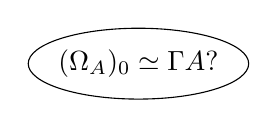
\begin{tikzpicture}\draw (0,0) ellipse (1.4 and .45);\node at (0,0) {$(\Omega_A)_0\simeq\Gamma A$?};\end{tikzpicture}}}

Dans le cas où $A=k$, on trouve $\Omega\simeq k[T]$, où les \inserted{additions,} multiplications et compositions sont celles des polynômes.
Dans ce cas, la condition $3^\circ)$ \unsure{s. les satisf.|satisf. aussi}.
Anneau des constantes est $k$.

On pourra aussi prendre $k[[T]]^+$, avec produit et $x\circ y$,
(l'anneau des ctes est réduit à zero / ou les $a_0+a_1T+\cdots$ avec $a_0$ \uline{nilpotent}
\margin{\unsure{Considérons} \uline{les \unsure{Schémas}} ou ``\uline{\unsure{Anneaux}}'' sur $k$ \uline{\unsure{pro-unip.}}}

\hrule
Soit $\Omega$ un analyseur, $\Omega_0$ le ps.-anneau des ctes, alors
\[
F\longmapsto(\lambda\longmapsto F\circ\lambda):
\Omega\longrightarrow\mathrm{App}(\Omega_0,\Omega_0)=\Omega_{\Omega_0}.
\]
est un ``homo d'analyseurs'', induisant une isom. sur les sous-\inserted{ps.}anneaux des constantes.
On est content quand
\[
\Omega\longrightarrow\deleted{\mathrm{App}}\Omega_{\Omega_0}
\quad\text{est injectif!}
\]
\margin{7}

\scanpage{9}
\begin{tabular}{l}
\texttt{\ STMT\ NO.\ MESSAGE} \\
\texttt{-} \\
\texttt{\ \ \ \ 4\ \ \ \ \ IEF653I\ SUBSTITUTION\ JCL\ -\ PGM=CRBATCH,REGION=100K,PARM=} \\
\texttt{\$HASP373\ STARTED\ -\ INIT\ 10\ -\ CLASS\ Q\ -\ SYS\ E333} \\
\texttt{IEF236I\ ALLOC.\ FOR\ PREDONTA\ CSSBATCH\ CRAY} \\
\texttt{IEF237I\ 581\ \ ALLOCATED\ TO\ STEPLIB} \\
\texttt{IEF237I\ 2C9\ \ ALLOCATED\ TO\ SYS00024} \\
\texttt{IEF237I\ VIO\ \ ALLOCATED\ TO\ SYSUT1} \\
\texttt{IEF237I\ JES2\ ALLOCATED\ TO\ SYSUDUMP} \\
\texttt{IEF237I\ 59F\ \ ALLOCATED\ TO\ CRJIF} \\
\texttt{IEF237I\ JES2\ ALLOCATED\ TO\ SYSIN} \\
\texttt{IEF237I\ 59F\ \ ALLOCATED\ TO\ SYS00002} \\
\texttt{IEF237I\ 59F\ \ ALLOCATED\ TO\ SYS00001} \\
\texttt{IEF285I\ \ \ CRAY1.PREDONT.CSS.D82109.T171033.R70\ \ \ \ \ \ \ \ CATALOGED} \\
\texttt{IEF285I\ \ \ VOL\ SER\ NOS=\ CRAY11.} \\
\texttt{CSS2060\ -\ JOB\ QUEUED\ FOR\ TRANSFER} \\
\texttt{IEF142I\ PREDONTA\ CSSBATCH\ CRAY\ -\ STEP\ WAS\ EXECUTED\ -\ COND\ CODE\ 0000} \\
\texttt{IEF285I\ \ \ CISI.PROD.CSSBATCH.V1.YY01\ \ \ \ \ \ \ \ \ \ \ \ \ \ \ \ \ \ KEPT} \\
\texttt{IEF285I\ \ \ VOL\ SER\ NOS=\ MVS104.} \\
\texttt{IEF285I\ \ \ SYSCTLG.VSAC015\ \ \ \ \ \ \ \ \ \ \ \ \ \ \ \ \ \ \ \ \ \ \ \ \ \ \ \ KEPT} \\
\texttt{IEF285I\ \ \ VOL\ SER\ NOS=\ SAC015.} \\
\texttt{IEF285I\ \ \ SYS82109.T171031.RA000.PREDONTA.SYSUT1\ \ \ \ \ \ DELETED} \\
\texttt{IEF285I\ \ \ JES2.JOB00026.S00102\ \ \ \ \ \ \ \ \ \ \ \ \ \ \ \ \ \ \ \ \ \ \ SYSOUT} \\
\texttt{IEF285I\ \ \ SYS1.CR.JIF\ \ \ \ \ \ \ \ \ \ \ \ \ \ \ \ \ \ \ \ \ \ \ \ \ \ \ \ \ \ \ \ KEPT} \\
\texttt{IEF285I\ \ \ VOL\ SER\ NOS=\ CRAY11.} \\
\texttt{IEF285I\ \ \ JES2.JOB00026.SI0101\ \ \ \ \ \ \ \ \ \ \ \ \ \ \ \ \ \ \ \ \ \ \ SYSIN} \\
\texttt{IEF285I\ \ \ SYSCTLG.VCRAY11\ \ \ \ \ \ \ \ \ \ \ \ \ \ \ \ \ \ \ \ \ \ \ \ \ \ \ \ KEPT} \\
\texttt{IEF285I\ \ \ VOL\ SER\ NOS=\ CRAY11.} \\
\texttt{IEF373I\ STEP\ /CSSBATCH/\ START\ 82109.1710} \\
\texttt{IEF374I\ STEP\ /CSSBATCH/\ STOP\ \ 82109.1710\ CPU\ \ \ \ 0MIN\ 00.16SEC\ SRB\ \ \ \ 0MIN\ 00.02SEC\ VIRT\ \ \ \ 84K\ SYS\ \ \ \ 240K} \\
\texttt{IEF375I\ \ JOB\ /PREDONTA/\ START\ 82109.1710} \\
\texttt{IEF376I\ \ JOB\ /PREDONTA/\ STOP\ \ 82109.1710\ CPU\ \ \ \ 0MIN\ 00.16SEC\ SRB\ \ \ \ 0MIN\ 00.02SEC}
\end{tabular}
\margin{8}

\scanpage{10}
\mspage{5}
\uline{Ex 2} Relatif: un couple $k_0\subset K_0$ d'anneaux commutatifs,
\[
\Omega\subset K_0[T],\qquad
\Omega=\{P\in K_0[T]\mid P(\lambda)\in k_0\quad\forall\lambda\in k_0\}
\]
structures $+,\cdot,\circ$ induites par celles de $K_0[T]$.
Le cas le plus intéressant est celui du couple $(\mathbb Z\subset\mathbb Q$:

\uline{L'analyseur binomial}\qquad (unitaire)

\inserted{\uline{Ex 3}\quad Analyseur des $\lambda$-anneaux (unitaire).}

\uline{Ex \unsure{4|5}}\quad Analyseur des puissances divisées (pas unitaire)
\figure{\begin{tikzpicture}\draw[->] (0,-1) .. controls (-1,-.3) and (-1,.45) .. (.25,.8);\end{tikzpicture}}
\margin{9}

\scanpage{11}
\begin{tabular}{rll}
\texttt{1} & \texttt{//PREDONTA\ JOB\ '*********,000000000','\ \ \ \ \ \ \ \ \ \ \ \ \ \ \ \ \ \ \ \ ',} & \texttt{JOB\ 0026} \\
\texttt{} & \texttt{//\ MSGLEVEL=(1,1)} & \texttt{} \\
\texttt{2} & \texttt{//CRAY\ \ \ \ \ EXEC\ CSSBATCH} & \texttt{00000040} \\
\texttt{3} & \texttt{XXCSSBATCH\ PROC\ REG=100K,P=''} & \texttt{00010000} \\
\texttt{4} & \texttt{XXCSSBATCH\ EXEC\ PGM=CRBATCH,REGION=\&REG,PARM=\&P} & \texttt{00020000} \\
\texttt{5} & \texttt{XXSTEPLIB\ \ DD\ DSN=CISI.PROD.CSSBATCH.V1.YY01,DISP=SHR} & \texttt{00030003} \\
\texttt{6} & \texttt{XXSYSUT1\ \ \ DD\ DSN=\&\&SYSUT1,UNIT=\unsure{SYSTS0|SYSTSO},SPACE=(TRK,30),DISP=(NEW,DELETE)} & \texttt{00031006} \\
\texttt{7} & \texttt{XXSYSUDUMP\ DD\ SYSOUT=*} & \texttt{00040000} \\
\texttt{8} & \texttt{XXCRJIF\ \ \ \ DD\ DSN=SYS1.CR.JIF,DISP=SHR} & \texttt{00050000} \\
\texttt{9} & \texttt{XXSYSIN\ \ \ \ DD\ DDNAME=CRAYIN} & \texttt{00060000} \\
\texttt{10} & \texttt{//CRAYIN\ \ \ DD\ *} & \texttt{00000050}
\end{tabular}
\margin{10}

\cotefile{155}
\scanpage{1}
\figure{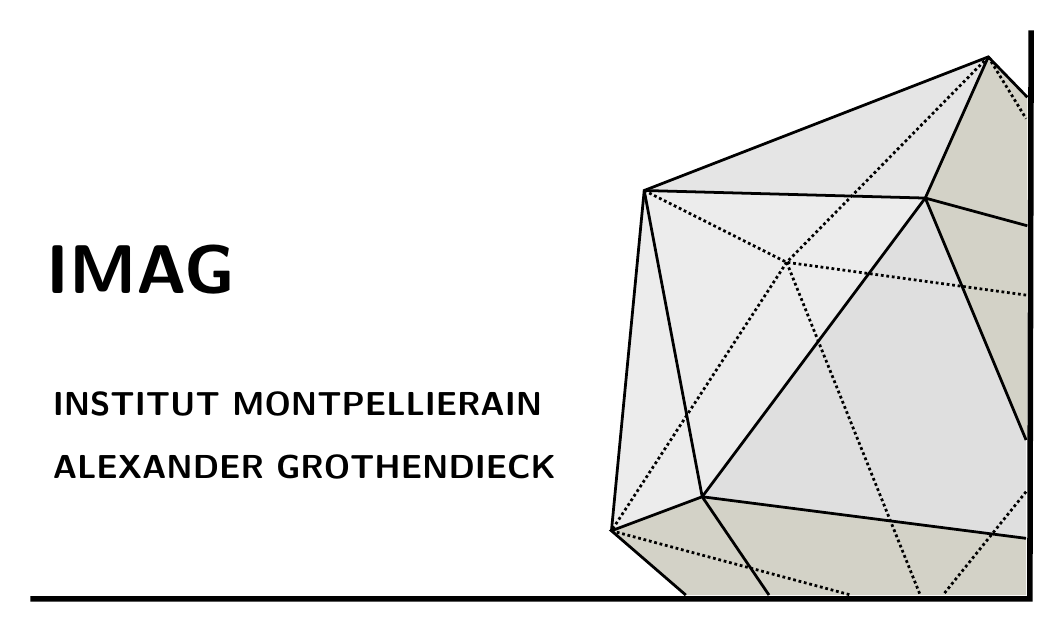
\begin{tikzpicture}[x=.016cm,y=.016cm]
\node[anchor=west,font=\sffamily\bfseries\fontsize{60}{65}\selectfont] at (15,285){IMAG};
\node[anchor=west,font=\sffamily\bfseries\large] at (20,179){INSTITUT MONTPELLIERAIN};
\node[anchor=west,font=\sffamily\bfseries\large] at (20,129){ALEXANDER GROTHENDIECK};
\fill[gray!20] (497,348)--(770,454)--(720,342)--cycle;
\fill[gray!15] (497,348)--(720,342)--(543,105)--(471,78)--cycle;
\fill[gray!25] (720,342)--(800,150)--(800,72)--(543,105)--cycle;
\fill[yellow!12!gray!45] (770,454)--(801,422)--(801,150)--(720,342)--cycle;
\fill[yellow!12!gray!45] (471,78)--(543,105)--(800,72)--(800,27)--(530,27)--cycle;
\draw[line width=1pt] (471,78)--(497,348)--(770,454)--(801,422);
\draw[line width=1pt] (497,348)--(720,342)--(801,320);
\draw[line width=1pt] (770,454)--(720,342)--(800,150);
\draw[line width=1pt] (497,348)--(543,105)--(596,27);
\draw[line width=1pt] (720,342)--(543,105)--(471,78)--(530,27);
\draw[line width=1pt] (543,105)--(800,72);
\draw[densely dotted,line width=1pt] (497,348)--(610,291)--(800,265);
\draw[densely dotted,line width=1pt] (770,454)--(610,291)--(471,78);
\draw[densely dotted,line width=1pt] (610,291)--(716,27);
\draw[densely dotted,line width=1pt] (471,78)--(661,27);
\draw[densely dotted,line width=1pt] (800,109)--(734,27);
\draw[densely dotted,line width=1pt] (770,454)--(800,405);
\draw[line width=2pt] (10,24)--(803,24)--(804,475);
\end{tikzpicture}}

\scanpage{2}
\mspage{1}
Soient $k$ un corps, $k'/k$ ext. finie.

La donnée d'une $\otimes$-catégorie Abel $C$ sur $k$,
et d'un \deleted{foncteur fibre (exact) \unsure{qui est} \uline{fidèle}}
$\otimes$-foncteur $k$-lin. Abel \deleted{exact et} \uline{fidèle}
\[
F:C\longrightarrow\mathrm{Modf}(k')
\]
équivaut à la donnée

1°) d'un schéma affine $G'$ sur $k'$, muni d'une section $\varepsilon$,
i.e. d'une $k'$-alg. comm. $U$, \deleted{\unsure{munie}}
$k'$-augmentée par $\varepsilon:U\unsure{\rightharpoondown|\longrightarrow} k'$.

2°) Sur le pro-objet $A=U^\vee
\inserted{\overset{\mathrm{def}}{=}\operatorname{Hom}_{k'}(U,k')}$
\deleted{de $\mathrm{Modf}(k')$}, considéré comme un pro-objet de
$\mathrm{Modf}(k)$, une structure de \deleted{\unsure{groupe}}
anneau associatif, admettant $\varepsilon$ comme unité,

avec les conditions suivantes

(i) L'hom $k'$-lin. $\lambda\mapsto\lambda\varepsilon\quad k'\unsure{\mathrel{-}|\longrightarrow} A$
est multiplicatif,
\inserted{\unsure{i.e.} la structure de pro-anneau de $A$ \uline{prolonge} celle de $k'$.}

\margin{\deleted{\unsure{Ab.}} (Comp.) $\left\{\vphantom{\begin{matrix}i\\ii\end{matrix}}\right.$}

(ii) l'hom \inserted{$k'$-lin.}
\[
A\longrightarrow A\widehat\otimes_{k'}A
\]
dual à la multiplication dans $U$ est ``multiplicatif'' i.e. prend ses valeurs
dans
\[
\underbrace{\widetilde J/J}_{\text{anneau}}\subset A\widehat\otimes_{k'}A
\quad
\left(
J=\mathfrak j\cdot
\underbrace{(A\widehat\otimes_k A)}_{\substack{\text{pro-}k\text{-alg. prod.}\\\text{tens.}}},
\ \text{idéal à droite eng. par }\
\mathfrak j=\ker(k'\otimes_k k'\longrightarrow k')
\right.
\]
\[
\widetilde J=\{\lambda\in A\widehat\otimes_k A\mid\lambda J\subset J\}
\]
et à ce titre est \deleted{\unsure{multip.}}
hom d'anneaux $A\longrightarrow\widetilde J/J$.
\margin{1}

\scanpage{3}
\begin{flushright}- 6 -\end{flushright}

L'auteur garantit à l'éditeur la jouissance totale et libre de toutes servitudes de ces droits, ainsi qu'il l'a fait pour le droit de publication en librairie, contre tous troubles, revendications ou évictions quelconques.

L'éditeur cessionnaire des droits ci-dessus s'emploiera, dans toute la mesure de ses moyens, à les exploiter au mieux de l'intérêt réciproque des parties, la non exploitation de l'un ou de plusieurs de ces droits ne pouvant en aucun cas être une cause de résiliation du présent contrat. L'éditeur assurera l'exploitation des droits dans les conditions propres à permettre à l'auteur la protection de son droit moral.

L'auteur s'engage à communiquer à l'éditeur toutes demandes qui lui seraient adressées par un tiers en vue d'une acquisition des droits sur l'œuvre pour toute adaptation, reproduction ou représentation.

\uline{9 - COMPTES}

Les comptes de l'ensemble des droits dus à l'auteur seront arrêtés une fois l'an, le premier avril de chaque année. Ils seront remis et réglés à l'auteur dans les trois mois suivant la date de leur arrêté. Les sommes payées seront considérées comme des avances pouvant être rectifiées ultérieurement d'après le compte des exemplaires en retour. En même temps que son arrêté annuel de comptes, l'éditeur remettra à l'auteur un état mentionnant le nombre d'exemplaires fabriqués en cours d'exercice et précisant la date et l'importance des tirages et le nombre d'exemplaires en stock. Cet état mentionnera également le nombre d'exemplaires vendus par l'éditeur, celui des exemplaires \unsure{inutilisables}, ou détruits par cas fortuit ou de force majeure.

L'éditeur s'engage à fournir à l'auteur toute justification permettant le contrôle des versements effectués.

\margin{-}
\deleted{\uline{10 - DROIT DE PREFERENCE}

Pour les œuvres qu'il se proposerait de publier dans l'avenir, soit sous son nom, soit sous un pseudonyme ou une marque quelconque, l'auteur accorde à l'éditeur, à dater du présent contrat, un droit de préférence aux conditions du présent contrat.

Ce droit sera exercé dans les conditions prévues à l'article 34 de la loi du 11 mars 1957 sur la propriété littéraire et artistique, et il est limité d'un commun accord à cinq ouvrages nouveaux, à compter de la signature du présent contrat, du même genre que celui qui donne lieu à la signature du présent contrat, c'est-à-dire :

La cession de chaque œuvre que l'éditeur aura acceptée sera régie par l'ensemble des clauses, charges et conditions du présent contrat, à l'exception de cet article lui-même, étant précisé qu'en cas de présentation simultanée et multiple d'ouvrages, l'éditeur fixera lui-même le délai de réalisation de chacun des ouvrages selon les usages de la profession et en tenant compte de l'intérêt commun des parties.}
\margin{-}
\margin{2}

\scanpage{4}
\mspage{2}
\uline{Ex}\qquad $C:\mathrm{Modf}(k)$\qquad
$F$ est le foncteur $M\otimes_k k'$.

Alors
\[
U=k'\otimes_k k'
\]
(structure de $k'$-alg. provenant du facteur gauche),
section canonique $\varepsilon:k'\otimes k'\longrightarrow k'$,
donc
\[
U^{\vee(k')}=A\simeq k'\otimes_k {k'}^{\vee(k)}
\simeq\operatorname{End}_k(k'),
\]
et on y prend la structure d'anneau habituelle.

\margin{\uline{NB} \unsure{alors}
\inserted{(si $k'/k$ est \unsure{ét.|étale}, donc $U\simeq A^{\vee(k)}$)}
$U\xrightarrow{\Delta_U}U\otimes_k U$ transposé de
$A\otimes_k A\longrightarrow A$ \unsure{est une}
\deleted{\unsure{structure}} \unsure{coalg.} \uline{\unsure{co-}}associative
($\Delta_U(1)\ne1$ en général, et $\Delta_U$ pas multiplicatif\ldots)}

\par\noindent\rule{.85\linewidth}{.4pt}\par
On cherche conditions \inserted{intrinsèques} sur \inserted{la $\otimes$-cat.} $C$ qui
assurent que pour \deleted{\unsure{$A\in C$}}
$k'/k$ et $F$ comme dessus, le foncteur des
$A_{\unsure{k'|k}}\inserted{=A\otimes_k k'}$-modules de \unsure{t.f.|d.f.}
\[
M'\longrightarrow M'\otimes_{k'\otimes_k k'}k'
\]
soit \uline{exact} (OK si $k'/k$ est étale) et \uuline{fidèle}.

Suffit il que $C$ soit \uline{rigide}, et que
\[
k\xrightarrow{\sim}\operatorname{End}_C(1_C)\quad???
\]
\par\hspace{.3\linewidth}\rule{.25\linewidth}{.4pt}\par
\uline{Exprimer la rigidité} de $C$ !
\margin{3}

\scanpage{5}
\begin{center}
UNIVERSITE DES SCIENCES ET TECHNIQUES\\
DU LANGUEDOC

\medskip
U.E. R. \quad 5
\end{center}

\bigskip
\begin{center}
\uline{D.E.A. DE MATHEMATIQUES}
\end{center}

\bigskip
Réunion d'information pour tous les étudiants

\medskip
\uline{Mercredi 10 octobre 1984 à 14h30, salle TD 33}

\bigskip
\begin{flushright}
P. MOLINO\\
Responsable 3e cycle
\end{flushright}
\margin{4}

\scanpage{6}
\mspage{3}
\uline{Rigidité}: $M\longrightarrow M^\vee$
\inserted{\deleted{\unsure{$=D(M)$}} $D(M)$}
compatible avec foncteur fibre $F'$,
foncteur équivalence de catégories, donc \uline{exact}
donc cont. à droit, \deleted{\unsure{donc donné aussi}}
donc donné par
\[
M\longmapsto\operatorname{Hom}_A(M,I)
\]
$I$ objet de $C$, muni d'opération de $A$: g.
\[
I=\deleted{\unsure{U}}D(A)
\underset{\inserted{\text{compatibilité avec }F'}}{=}
A^{\vee(k')}=U
\]
avec opération à g. de $A$ provenant par transposition
des opérations de $A$ à droite sur $A_g$, donc $U$ est un $A$-module.

Il faut donc faire opérer $A$ à gauche sur cet objet de
$\operatorname{Mod}(A)$ (donc mettre sur $U$ une structure de
\deleted{bimodule} module sur
\[
\underbrace{A}_{\text{op. à définir}}\otimes
\underbrace{A}_{\text{opération déjà connue}}.
\]

\margin{\uline{NB}}

Or les endom de $U$ en tant que $A$-module à g.
\inserted{(attention, ils ne sont pas néc. $k'$-linéaires,
pour la $k'$-structure \unsure{donnée|dualité} sur $U$!)}
correspondent aux endomorphismes de $A$ en tant que $A$ module à droite:
\[
\operatorname{End}_A(U)\simeq
\operatorname{End}_A(A_d)^o\simeq A^o
\]
donc il faut se donner
\[
A\xrightarrow{a:u\mapsto\unsure{\check u|\widetilde u}}A^o
\]

\margin{\unsure{est-ce que} \unsure{n'est valable que|n'est valable} \unsure{si}
$k'/k$ \unsure{est fini}, \unsure{donc} pour identifier
$U$ à $D_k(A)$ $(\simeq D_{k'}(A))$}
\margin{5}

\scanpage{7}
\figure{
\begin{tikzpicture}[x=.75cm,y=.75cm]
\foreach \t/\x/\y/\r in {U/-2/0.6/48,N/-1.65/1.03/38,I/-1.23/1.3/24,V/-.85/1.48/16,E/-.4/1.57/5,R/.1/1.6/0,S/.6/1.52/-12,I/1.05/1.36/-23,T/1.45/1.12/-33,E/1.8/.77/-45}
{\node[rotate=\r] at (\x,\y) {\t};}
\node[align=center,font=\scriptsize\bfseries] at (0,.3) {ARTS et LETTRES\\LANGUES et SCIENCES\\HUMAINES};
\foreach \t/\x/\y/\r in {P/-2/-.05/-40,A/-1.65/-.4/-32,U/-1.2/-.63/-20,L/-.75/-.8/-12,V/-.15/-.92/0,A/.3/-.9/5,L/.75/-.78/16,E/1.15/-.57/25,R/1.55/-.3/37,Y/1.85/.06/48}
{\node[rotate=\r] at (\x,\y) {\t};}
\draw (-.5,-1.65)--(.5,-1.65);
\node at (0,-2.2) {MONTPELLIER};
\end{tikzpicture}}

\begin{flushright}
MONTPELLIER, le 11 JUILLET 1984

\medskip
LE VICE-PRESIDENT DE\\
L'UNIVERSITE PAUL VALERY\\
DELEGUE AUX RELATIONS INTERNATIONALES
\end{flushright}

\uline{Service des Etudiants Etrangers}

CL/MC/N° 658

\begin{flushright}
à

\medskip
Monsieur CANO\\
Vice-Président administrateur provisoire\\
MONTPELLIER II
\end{flushright}

\bigskip
Monsieur le Président,

Dans le cadre du resserrement du jumelage entre Montpellier et Barcelone, une délégation du Conseil Municipal de Montpellier conduite par le député-maire Georges FRECHE a été reçue à Barcelone les 22 et 23 Juin dernier par Monsieur MARAGALL, maire de la ville.

Invité à accompagner cette délégation au titre de vice-président délégué aux Relations Internationales de l'Université Paul Valéry, j'ai participé à une réunion de travail présidée par M. Georges FRECHE et réunissant les vice-recteurs de l'Université Polytechnique de Catalogne, l'Université Centrale et l'Université autonome de Barcelone et l'Attaché Culturel directeur de l'Institut français de Barcelone.

Au cours de cette réunion, il a été décidé d'un commun accord de renforcer les relations pédagogiques et scientifiques entre les Universités de Barcelone et les Universités de Montpellier.

Pour ce faire, il a été convenu de recenser auprès de chaque Université les secteurs qui font déjà l'objet d'échanges entre les deux villes, ou ceux dans lesquels un travail en commun s'annoncerait fructueux. En effet, une collaboration efficace et durable entre universités repose sur une volonté et un besoin d'approfondir ensemble une activité de recherche.

A la suite de ce recensement, une rencontre des représentants des universités des deux villes sera organisée à Montpellier à l'automne 1984.

\begin{flushright}\ldots/\ldots\end{flushright}

\bigskip
Route de Mende - Boite Postale 5043 - 34032 MONTPELLIER C E D E X - Tél. (67) 63. 91. 10
\margin{6}

\scanpage{8}
\mspage{4}
\uline{NB}
\[
\inserted{D(M)=}
\operatorname{Hom}_A(M,U_g)
=\operatorname{Hom}_A(M_g,\operatorname{Hom}_{k'}(A_g,k'))
\]
\[
\simeq\deleted{\unsure{A_g}}\quad
\text{module des homs }k\text{-bil.}\quad
A_g\times M_g\overset{\varphi}{-}k'
\]
telles que
\[
\begin{aligned}
\varphi(\lambda u,x)&=\lambda\varphi(u,x)\\
\varphi(u\deleted{\unsure{\otimes}}v,x)&=\varphi(u,v.x)
\end{aligned}
\qquad
\begin{gathered}
\lambda\in k'\\u\in A\\x\in\unsure{u|M}
\end{gathered}
\]
i.e. correspondent aux homs
\[
A_d\otimes_A M\longrightarrow k'
\]
qui sont $k'$-linéaires, pour la structure de $k'$-module à gauche
provenant de $A_d$.

Or
\[
\begin{aligned}
A_d\otimes_A M&\xleftarrow{\sim}M
&&\text{isom de }k'\text{-modules}\\
1\otimes x&\mathrel{\longleftarrow\!\vert} x\\
\lambda(1\otimes x)=\lambda\otimes x=1\otimes\lambda x
&\mathrel{\longleftarrow\!\vert}\lambda x
\end{aligned}
\]
donc on trouve bien \deleted{\unsure{$M^{\vee(k')}$}}
\[
F'(D(M))=M^{\vee(k')}
\]
et la donnée de $a:A-A^o$ permet de mettre sur
$M^{\vee(\unsure{k'|k})}$ une structure de $A$-module.

Il faut encore que
\[
\deleted{\unsure{M\otimes M^{\vee(k')}}}
\]
\[
\underbrace{F'(M)}_{\substack{\deleted{\unsure{F'(M)}}\\
M_{\deleted{\unsure{k'}}}^{k'}}}
\otimes
\underbrace{F'(D(M))}_{(M^{k'})^\vee}
\longrightarrow k'=F'(1_C)
\]
provient bien \deleted{$A$} d'un hom
\[
M\otimes D(M)\longrightarrow1_C
\]
\margin{7}

\scanpage{9}
\begin{center}
UNIVERSITE DES SCIENCES ET TECHNIQUES\\
DU LANGUEDOC\\
Institut de Mathématiques
\end{center}
\begin{flushright}N° 2\end{flushright}

\begin{center}
Procés-Verbal de la réunion du 17 juillet 1984

\uline{de la COMMISSION DE SPECIALITE D'ETABLISSEMENT N°5}

\uline{``Constituants élémentaires, astronomie''}
\end{center}

Réunion à 14 h, salle 331, batiment de Mathématiques.

PRESENTS : MM. ANDRILLAT, AUBERSON, CECCHI, LOUPIAS, MENNESSIER, SABATIER,\\
\hspace*{2cm}MM. CUER, GLEIZES, JAULENT, BAYER, CORDONI.

EXCUSES : MM. CAPDEQUI PEYRANERE, MAS.

Après énoncé du problème posé (propositions de nomination sur un poste d'assistant susceptible d'être vacant, 30 e section) et rappel des conditions particulières apparues lors de la création de cette vacance (permettre de régler le problème d'un délégué en position d'attente depuis plusieurs années), M. SABATIER indique le nom des candidats, afin que les présents sachent s'ils sont ou non leurs parents. Il dresse ensuite un tableau des renseignements succincts sur les 13 candidatures reçues, savoir : M. ADAM \unsure{Dominique}, M. CORTEGGIANI Jean Pierre, M. BONNAREL François, M. FRANGI Jean Pierre, M. GERLAND Jean Michel, M. GIRAUD Edmond, M. GLEYSE Bernard, M. MONIER Richard, M. NITSCHELM Christian, M. POCHET Jean Marie, M. RANDON Jacques, M. REBOUL Henri, Mle \unsure{REMY} Frédérique. Ces renseignements sont complétés par les rapporteurs, de façon très détaillée pour les meilleurs candidats. M. SABATIER expose ensuite les conditions de vote et on procède à celui-ci, ligne par ligne. Pour 11 votants, la majorité absolue étant atteinte à 6, les résultats obtenus ont permis de proposer chaque fois par vote acquis au 1er tour,

en première ligne : M. REBOUL (11 bulletins Reboul)\\
en deuxième ligne : M. GIRAUD (6 Giraud, 2 Rémy, 1 Adam, 2 blancs),\\
en troisième ligne : Mle REMY (7 Rémy, 1 Adam, 3 blancs).

A 15 h 45 la séance a donc été levée.

\begin{flushright}P. SABATIER\end{flushright}
\margin{8}

\scanpage{10}
\mspage{5}
i.e. que
\[
M^{k'}\otimes_{k'}(M^{k'})^\vee\longrightarrow k'
\]
est $A$-linéaire, pour la \inserted{$A$} structure
diagonale. Il suffit de le prouver pour $M=A$
\diagram{
\begin{tikzcd}[ampersand replacement=\&,row sep=3.5em,column sep=large]
A^{k'}\otimes_{k'}U\arrow[r,"{\text{acc. can.}}"]\&
\unsure{k^{\wedge}|k'}\\
A\otimes\unsure{\,;}\arrow[u,dash]\&
\end{tikzcd}
}
\margin{9}

\scanpage{11}
UNIVERSITE DES SCIENCES ET\\
TECHNIQUES DU LANGUEDOC\\
Institut de Mathématiques

\begin{flushright}Montpellier, le 5 juin 1984\end{flushright}

Cher Collègue,

J'ai accepté d'être le responsable local, pour les mathématiques, du ``Congrès National des Sociétés Savantes'' qui se tiendra à Montpellier pendant les vacances de Pâques 1985. Le Responsable National en est Monsieur DUBREIL.

Ce congrès comportera, entre autre chose, une journée mathématique qui offre la possibilité d'une publication rapide sous forme d'un fascicule offset de 100 à 150 pages, sortant vers la fin de l'année.

Le programme comprend : d'une part des communications originales d'environ 25 minutes chacune ; d'autre part 2 ou 3 conférences de 50 minutes, dont l'une peut faire l'objet d'un rapport synthétique sur une question dont il est souhaitable de faciliter l'accès aux non-spécialistes.

Chaque auteur reçoit gratuitement 30 \unsure{tirés} à part.\\
Il est prévu que l'accent doive être mis plutôt sur l'algèbre, mais toute autre partie des mathématiques peut faire l'objet d'un exposé.

Malgré l'apparent confort des délais, il serait souhaitable que les Collègues qui seraient dès maintenant intéressés me le fassent savoir au cours de ce mois de juin 1984, en précisant le thème prévu de leur communication.

Je les en remercie d'avance.

\begin{flushright}N. ROBY\end{flushright}
\margin{10}
